% Whole document compilation
\newcommand{\setflag}{\newif \ifwhole \wholetrue}

% \usepackage{helvet}
% \renewcommand{\familydefault}{\sfdefault}

\newif\ifsans%
\sanstrue%

\ifsans%
\documentclass[11pt,a4paper,notitlepage,twoside,openright]{report}
\usepackage[sfdefault]{FiraSans}
\usepackage{FiraMono}
\usepackage{arevmath}
\else%
\documentclass[12pt,a4paper,notitlepage,twoside,openright]{report}
\fi%

\usepackage{adjustbox} % Rotated table headers
\usepackage{array} % Rotated table headers
\usepackage{booktabs} % Nice tables
\usepackage[headheight=15pt, top=1.1in, bottom=1.25in, left=1.25in, right=1.25in]{geometry} % 15pt for fancyhdr
\usepackage{docmute}  % For including stand-alone LaTeX documents as is
\usepackage{enumitem} % For referrable enumerated lists
\usepackage{fancyhdr} % Fancy headers
\usepackage[T1]{fontenc}
\usepackage[pdftitle={Exploring the structure of mathematical theories using graph databases},
            pdfauthor={Dhruv Makwana},
            pdfkeywords={mathematics, theorem, prover, graph, database, structure}]{hyperref} % (hyper)links
\usepackage[utf8x]{inputenc}
\usepackage[outputdir=build]{minted} % Source code highlighting
\usepackage{minitoc}  % Per Chapter Mini Table of Contents (load after)
\usepackage{pgfplots} % Graphs
\usepackage{titlesec} % For customising chapter titles
\usepackage{xcolor} % More colour names

% Formatting to allow flexible pages 
\raggedbottom{}
\sloppy
% penalise orphan lines/paragraphs
\clubpenalty1000%
\widowpenalty1000%

% Paragraph formatting
\parindent0pt%
\parskip6pt%

% Remove ugly boxes around hyperlinks
\hypersetup{%
    colorlinks,
    linkcolor={black},
    citecolor={green!50!black},
    urlcolor={blue!80!black}
}

% Include pink book guidance or not
\newif\ifguidance%
\guidancefalse%
\newcommand{\guidance}[1]{%
  \ifguidance%
  \textsf{\color{red}{#1}}
  \newpage
  \fi%
}%

% Fancy (and smaller) chapter heading style
\titleformat{\chapter}[hang]{\Huge\bfseries}{%
\thechapter\hspace{20pt}\textcolor{lightgray}{|}\hspace{20pt}}{0pt}{\Huge\bfseries}

% At the start of each chapter
\renewcommand{\mtctitle}{}
\newcommand*{\prechapter}[1]{%
\minitoc%
\bigskip%
\begin{center}%
  \begin{minipage}[h][][c]{0.8\linewidth}%
	#1
  \end{minipage}%
\end{center}

\newpage%
}

% Update MiniToC fonts
\ifsans%
\renewcommand{\mtifont}{\large\sffamily}
\renewcommand{\mtcfont}{\normalsize\sffamily}
\renewcommand{\mtcSfont}{\normalsize\sffamily\bf}
\renewcommand{\mtcSSfont}{\small\sffamily}
\renewcommand{\mtcSSSfont}{\small\sffamily}
\fi%

% Fancy evaluation table with slanted columns
% http://tex.stackexchange.com/questions/32683/rotated-column-titles-in-tabular#32690
\newcolumntype{R}[2]{%
    >{\adjustbox{angle=#1,lap=\width-(#2)}\bgroup}%
    l%
    <{\egroup}%
}
\newcommand*\rot{\multicolumn{1}{R{90}{1em}}}%


\begin{document}

\pagestyle{empty}

\hfill{\Large \sffamily \bfseries Dhruv C.\ Makwana}

\vspace*{60mm}
\begin{center}
\Huge
{\sf \bfseries Exploring the structure \\ of mathematical theories \\ using graph databases} \\
\vspace*{5mm}
Computer Science Tripos, Part II \\
\vspace*{5mm}
Trinity College \\
\vspace*{5mm}
May 10, 2017
\end{center}

\cleardoublepage{}

\setcounter{page}{1}
\pagenumbering{roman}
\pagestyle{plain}

\chapter*{Proforma}

{%
\begin{tabular}{ll}
Name:               & \bf Dhruv Makwana \\
College:            & \bf Trinity College                     \\
Project Title:      & \bf Exploring the structure of mathematical theories \\
                    & \bf using graph databases \\
Examination:        & \bf Computer Science Tripos, Part II, 2016--2017 \\
Word Count:         & \bf 11,044 \\
Project Originator: & Dr.\ Timothy G. Griffin \\
Supervisor:         & Dr.\ Timothy G. Griffin \\
\end{tabular}
}

\section*{Original Aims of the Project}

This project aims to (a) represent Coq libraries as Neo4j (graph) databases and
(b) create a library of Neo4j tools with the goal of highlighting the structure
and relationship between the representations of the proof-objects.  It also
aims to have more features but still perform comparably to existing tools which
help a user understand a Coq library. As an extension, this project aims to
work with the Odd Order Theorem (part of Mathematical Components Coq library).

\section*{Work Completed}

This project represents Coq libraries as Neo4j (graph) databases and provides a
library of Neo4j tools that highlighting the structure of and relationship
between proof-objects. It performs comparably to existing tools which help a
user understand a Coq library. This project works with the Odd Order Theorem
(part of Mathematical Components Coq library) extension task.

\section*{Special Difficulties}
None.

\newpage
\section*{Declaration}

I, Dhruv Makwana of Trinity College, being a candidate for Part II of the
Computer Science Tripos, hereby declare that this dissertation and the work
described in it are my own work, unaided except as may be specified below, and
that the dissertation does not contain material that has already been used to
any substantial extent for a comparable purpose.

\bigskip
\leftline{\textbf{Signed}: Dhruv Makwana}

\bigskip
\leftline{\textbf{Date}:\date}

\cleardoublepage{}

\dominitoc% Initialisation
\setcounter{tocdepth}{1}
\tableofcontents
\cleardoublepage{}

\setcounter{page}{1}
\pagenumbering{arabic}
\pagestyle{fancy}

\chapter{Introduction}


\guidance{%
  The Introduction should explain the \textbf{principal motivation} for the
  project.  \textbf{Show how the work fits into} the broad area of surrounding
  Computer Science and \textbf{give a brief survey} of previous related work.
  It should \textbf{generally be unnecessary to quote at length} from technical
  papers or textbooks. If a simple bibliographic reference is insufficient,
  consign any lengthy quotation to an appendix.
}

\prechapter{%
  This dissertation offers a solution to problems regarding the presentation of
  mathematics. Firstly, these problems and the specific systems involved are
  described. Then, the aims of the project are stated; in later chapters, details
  of the prepration and implementation carried out are expounded. Lastly, the
  chapters on evaluation and conclusion provide evidence for the success of the
  project, reflections on the process and suggestions for future work.
}

\section{Problem}

Mathematics textbooks aimed at professionals/researchers follow a well-established
rhythm: define some constructions and some properties on them and prove
theorems on both, with lemmas, corollaries and notation interspersed
throughout. Such a presentation is concise but limiting: it is linear; it forces
the reader to keep track of dependencies such as implicit assumptions, previously
defined results and the types and conventions behind any notation used;
and it offers little opportunity to consider and compare different approaches
for arriving at a result (i.e.\ number of assumptions, number of steps, some
notion of the importance of a result such as number of uses by later
results).

With the increasing popularity of interactive proof-assistants such as
Coq~\cite{Coq:manual} and Isabelle~\cite{nipkow2002isabelle}, many mathematical
theories (such as the formidably large Feit-Thompson Odd Order
Theorem~\cite{peterfalvi2000oot, bender1994oot}) have
been~\cite{gonthier2013oot} or are being translated and formalised into
machine-checked proof-scripts. However, these proof-scripts on their own
inherit the same disadvantages as the aforementioned textbooks, as well as some
new ones: they are usually more verbose and explicit and are primarily designed
for automation/computation than readability. The former (usually out of
necessity to convey to the computer the intended meaning) leads to unnecessary
``noise'' in the proof and the latter departs from the vocabulary or flow of a
natural-language presentation.

The database world is currently experiencing a tremendous explosion of creativity
with the emergence of new data models and new ways of representing and querying
large data sets. \emph{Graph databases} have been developed to deal with highly
connected data sets and path-oriented queries. That is, graph databases are
optimised for computing transitive-closure and related queries, which pose a
huge challenge for traditional, relational databases.

\section{Solution}

A graph-based approach to the representation and exploration of the structure of
proof-objects would  be a far more natural expression of the complex
relationships (i.e.\ chains of dependencies) involved in
constructing mathematical theories. Questions such as ``What depends on this
lemma and how many such things are there?'' or ``What are the components of
this definition?'' could thus be expressed concisely (questions which are not
even expressible with standard relational databases systems such as
SQL). A popular graph database, Neo4j~\cite{neo4j} with an expressive query
language \emph{Cypher} will be used for this project.

\section{Coq Proof-Assistant}

The Coq proof-assistant -- implemented in OCaml -- can be viewed as both 
a system of logic -- in which case it is a realisation of the \emph{Calculus of
Inductive Constructions} -- and as a \emph{dependently-typed} programming
language. Its power and development are therefore most-suited and often geared
towards \emph{large scale} developments.

On the logical side, Coq lays claim to projects such as the Four-Colour
Theorem~\cite{gonthier2008formal} (60,000 lines) and the aformentioned
\emph{Feit-Thompson} theorem (approximately 170,000 lines, 15,000
definitions and 4,200 theorems) are feats of modern software-engineering.

On the programming language side, Coq has served as the basis for many equally
fantastic projects. The \emph{CompCert Verified C
Compiler}~\cite{leroy2012compcert} demonstrates the practical applications of
theorem-proving and dependently-typed programming by implementing and proving
correct an optimising compiler for the C programming language.
\emph{DeepSpec}~\cite{pierce2016science}, a recently announced meta-project,
aims to integrate several large projects such as \emph{CertiKOS} (operating
system kernels, \emph{Kami} (hardware), \emph{Vellvm} (verifying LLVM) and many
more in the hopes to provide complete, \emph{end-to-end} verification of
real-world systems.

\section{Neo4j Database and the Cypher Language}

Neo4j is a graph database system implemented in Java. Traditional, relational
database theory and systems are designed with the goal of storing and
manipulating information in the form of \emph{tables}. As such, working with
highly interconnected data, such as social network graphs is best tackled with
the alternative approach of \emph{graph databases}.

Briefly, a (directed) \emph{graph} is defined as $G = (V, E)$ where $V$ is a set
of vertices or \emph{nodes} and $E \subseteq V \times V$ is a set of edges or
\emph{relationships} between two nodes. A \emph{graph database} is an OLTP
(online transaction processing, meaning operated upon live, as data is
processed) database management system with CRUD (create, read, update and delete)
operations acting on a graph data model. Relationships are therefore promoted to
first-class citizens and can be manipulated and analysed.

\subsection{Cypher: An Illustrated Example}

\emph{Cypher} features heavy use of pattern-matching in an ASCII-art inspired
syntax.  The following (slightly contrived but hopefully illuminating) example
in Listing~\ref{lst:cypherexample} illustrates some of the key strengths of
graph-based modelling using Cypher. 

Suppose we have a puppy named ``Cliff'' looking for the nearest and most
familiar children (for this example, a person under the age of six) to play
with.

To see how Cliff (indirectly) likes/knows this child, we bind \emph{path} to the
result of the \emph{shortestPath} query.  For the path itself, we start with a
node following this structure: \mintinline{cypher}{(var:label {attrib: val})}.
We then have a \emph{labeled, transitive} relationship (explicitly limiting our
search to paths of up to length four) expressed as an arrow with a label
\texttt{-[..]->}. As such, we can discard any paths with relationships we do not
want (e.g.\ \texttt{HATES}). 

To filter based on more complex logic (than possible by pattern-matching directly
on labels and attributes) we can express the requirement that the age of a dog by
the name of Cliff be less than or equal to two (and similarly for the age of the
child) in the \mintinline{cypher}{WHERE} clause.

Lastly, we return the path and order the results by proximity as a row of
results, renaming the column of the child's name to simply ``name''.

\begin{listing}[tb]%

\caption{Example Cypher Query}\label{lst:cypherexample}

  \begin{minted}{cypher}
  MATCH path = shortestPath(
    (puppy:dog {name: "Cliff"})-[:LIKES|:KNOWS*..4]->(child:person))
  WHERE puppy.age <= 2 AND child.age < 6
  RETURN path,
         child.name AS name,
  ORDER BY other.distance_from_clifford
  \end{minted}

\end{listing}

\section{Related Work}

Some existing tools offer part of the solutions.%

dpdgraph
(\href{http://github.com/Karmaki/coq-dpdgraph}{\texttt{github.com/Karmaki/coq-dpdgraph}})
is a tool which analyses dependencies between \emph{compiled} Coq proofs. As
such, desirable information about notation, tactics, definitions and the
relationship between a type and its constructors is lost.

Coqdep is a utility included with Coq which analyses dependencies \emph{at the
module level} by tracking {\tt Require} and {\tt Import} statements.

Coq SerAPI
(\href{http://github.com/ejgallego/coq-serapi}{\texttt{github.com/ejgallego/coq-serapi}})
is a work-in-progress library and communication protocol for Coq designed to
make low-level interaction with Coq easier, especially for IDEs. It has a
starting point for gathering some statistics of proof-objects in a project.

\section{Aims of the Project}\label{intro:aims}

This project aims to:

\begin{itemize}
\item represent Coq libraries as Neo4j graph databases, which wil involve
  \begin{itemize}
  \item exploring and choosing the correct model
  \item converting and extending existing code to output CSVs
  \item writing new programs to extract extra information \\
      (omitted from other, existing tools)
  \item writing new programs to automate database creation; and to
  \end{itemize}

\item create a library of Neo4j queries, intended
  \begin{itemize}
  \item to highlight the structure of and relationship between proof-objects
  \item by coalescing and implementing several graph-related metrics.
  \end{itemize}
\end{itemize}

\section{Summary}

An explanation of the problems which conventional presentations of mathematics
suffer from was given, with \emph{graph databases} proposed as a solution. 
Existing tools were mentioned and the requirements for a successful project
were listed.


\chapter{Preparation}

{\sf \color{red}
  Principally, this chapter should \textbf{describe the work which was
  undertaken before code was written}, hardware built or theories worked on. It
  should \textbf{show how the project proposal was further refined and
  clarified}, so that the Implementation stage could go smoothly rather than by
  trial and error.

  Throughout this chapter and indeed the whole dissertation, it is essential to
  \textbf{demonstrate that a proper professional approach was employed}.

  The nature of this chapter will vary greatly from one dissertation to another
  but, underlining the professional approach, this chapter will very likely
  include a \textbf{section headed “Requirements Analysis”} and
  \textbf{incorporate other references to the techniques of Software
  Engineering}.

  The chapter will cite any \textbf{new programming languages and systems which
  had to be learnt} and will \textbf{mention complicated theories or
algorithms} which required understanding.

  It is essential to \textbf{declare the Starting Point} (see Section 7). This
  states \textbf{any existing codebase or materials} that your project builds
  on.  The text here \textbf{can commonly be identical to the text in your
  proposal}, but it may \textbf{enlarge on it or report variations}. For
  instance, the true starting point may have turned out to be different from
  that declared in the proposal and \textbf{such discrepancies must be
  explained}.
}

Before commencing implementation of the project, careful consideration was
given to planning it. Current solutions were explored, studied and evaluated
against the aims described in Section~\ref{intro:aims}. The rest of this
chapter will explain the initial set-up, elaborate on findings concerning
related work and outline the project's starting point.

\section{Project Planning}

This project presents a unique idea and breaks new ground. As such, the
methodology had to suit and reflect the largely exploratory nature of the
process. A spiral software development model was chosen: think of an idea,
modify the model (of Coq proof-objects), implement and propogate the necessary
changes, evaluate the end-result and repeat. This allowed for experimentation
of ideas and flexibility of implementation strategies.

Git (\href{http://git-scm.com}{\texttt{git-scm.com}}) and GitHub
(\href{http://github.com/dc-mak}{\texttt{github.com/dc-mak}}) were invaluable during the
project, allowing for easy tracking, reverting, reviewing and collaborating.
New features could be tested on new branches before being merged in and a copy
of the work was safely backed up in one more place. GitHub extensions such as
Travis-CI (continous integration) were added in later, as it became apparent
that precisely specified versioning, build-dependencies and automated tests were
useful in spotting errors early.

\section{Requirements Analysis}
Several components of this project needed to function correctly, both
individially and in conjuction for it to work. Separate parts for
modelling/translation (from Coq to the chosen model), displaying and
interacting (Neo4j/Cypher) and computation (Neo4j/Cypher plugins)
needed to be developed and brought together. Below is a list of required
features used throughout development to guide and provide context for
implementation decisions.

\begin{itemize}

  \item \textbf{Modelling}: The model should
  \begin{itemize}

    \item include as much relevant data as possible. Here, relevant means
          useful to understanding a large library, but not so much so as to
          obfuscate any information or make learning how to use the project
          more difficult.

    \item be flexible to work with and easy to translate. One could imagine
          different front-ends for interacting with and computing data
          from the model.

    \item strike a balance between size and precomputing too much data.
          Figuring out which pieces of data can be reconstructed later and
          which are beneficial to compute during modelling will be a matter of
          experimentation and weighing up ease of implementation
          versus ease of later processing.

  \end{itemize}

  \item \textbf{Interaction}: Interacting with the model should
  \begin{itemize}

    \item primarily, allow users to understand the data. The following two points
          follow from this principal goal.

    \item support both graphical and textual modes of use. Small queries and
          novice users are likely to benefit from the presence of a well-designed
          GUI. However, larger queries requiring more computation and
          flexibility will benefit from a traditional, shell-like interface.

    \item be interactive and extensible. A static presentation of data, even in
          a GUI, would fail to make full use of graph-databases and the ability
          to query, in whatever way the user desires, information dynamically.

  \end{itemize}

  \item \textbf {Computation}: Working with the model's data should
  \begin{itemize}

    \item be enabled by a core library of good defaults. Certain, common
          functions should be ready `out-of-the-box' and provide users
          all they need to get started.

    \item allow the user to add their own functions. It is not possible
          to imagine and implement all the functionality users may desire and
          so a way to extend the project to suit their own needs would be of
          great use.

  \end{itemize}


\end{itemize}

\section{Technologies Used}

Choice of implementation languages was, although an important decision, almost
completely dictated by the programs at the core of the project (Coq and Neo4j).

Coq and its plugins -- specifically, {\tt dpdgraph}, which was used as a
starting point for extracting information about Coq proof-objects from compiled
proof-scripts -- are written in OCaml
(\href{http://ocaml.org}{\texttt{ocaml.org}}).  Since it almost always wiser to
work with and modify existing sytems (and more representative of real-world
work) and as a functional language, OCaml benefits from strong, static (and
inferred) type-system (allowing for easy experimentation, greater confidence in
correctness), sticking to it for other parts of the tools which need not
necessarily be in OCaml (e.g.\ the {\tt dpd2csv} utility) was a welcome and
easy decision. OCaml has several other benefits too, such as
inductively-defined datatypes (useful for manipulating Coq constructs) and good
editing tools.

Similarly, Neo4j and its plugins are (usually) written in Java, but several
lanaguages are supported for the latter, both by Neo4j officially and by the
community. As will be explained in sub-section~\ref{subsec:neo4jandtools}, Java
and R were found to be the most suitable for achieving this project's goals.

\section{Starting Point}

\subsection{Coq}

Coq is a \emph{large} project, devloped by INRIA (France), and its size and
complexity are best experienced through detangling the source code for yourself.
Just for the implementation of the system (not including the standard library),
Coq features approximately 3 major ASTs, 6 transformations between them, 3000
visible types, 9000 APIs and 521 implementation files containing 228,000 lines
of dense, functional OCaml.

However, most of this massive project is sporadically (and tersely) documented.
Even after consulting the Coq developers' mailing-list, several hours were spent
browsing the source code to overcome the severe difficulties in understanding
the project. Prior familiarity with \emph{using} Coq (as an introduction
to tactical theorem-proving and dependently-typed programming) was not useful
for understanding the internals beyond context and how to compile and use
programs and libraries. However, it did serve as invaluable insight for
\emph{cognitive walkthroughs} carried out during the implementation phase
(as a structured way of guiding the design of the model and libraries).

\subsection{Existing Tools for Coq}
A number of tools were studied to learn their approaches and analyse their
strengths and weakeness. A full, detailed comparison between all the tools
mentioned and this project will be presented later, during evaluation.  What
follows is a brief overview of each tool and the reason it was insufficient for
the purposes of meeting the project aims and requirements.

\subsubsection{Coqdoc}
Coqdoc is a documentation tool for Coq projects. It can output to raw text,
HTML, \LaTeX~and a few other formats. Although it supports prettifying code with
syntax highlighting and unicode characters, its most relevant feature was its
hyperlinking: potentially useful for building dependency graphs.

However, the whole tool worked on an entirely \emph{lexical} level, with no
formal parsing, understanding or elaboration of the code structure. Some efforts
were made to modify its output into a useful format (e.g. comma-separated
values) for other tools; however these did not prove fruitful because
tokenisation cannot infer or preserve as much information as full compilation.
Hence, since it could not meet any of the modelling requirements (completeness,
flexibility and size/precomputation) this approach was abandoned.

\subsubsection{Coqdep}
Coqdep is a tool which computes inter-module dependencies for Coq and
OCaml programs, outputtting in a format readable by the \texttt{make} program.
Although on first impressions, this tool seemed to offer more flexibility than
coqdoc, it was even more restrictive: it simply searches for keywords such as
\texttt{Require} or \texttt{Import} for Coq  and \texttt{open} or dot-notation
module usage for OCaml) per file and outputs them accordingly.  As with coqdoc
(and for the same reasons), this approach was also abandoned.

\subsubsection{CoqSerAPI}

\emph{Coq Se(xp)rialized API} is a new library and communication protocol aiming to
make low-level interactions easier (using OCaml datatypes and s-expressions),
particularly for tool/IDE developers. While this is likely to be useful in the
future, it is still far from complete and is more geared towards interactive
\emph{construction} (via a tool/IDE) rather than \emph{analysis}. As such,
tracking dependencies (critical to the modelling requirements) is not possible.

\subsubsection{dpdgraph}

dpdgraph is a tool which extracts dependencies between Coq objects from compiled
Coq object-files to a \texttt{.dpd} file. It includes two example tools:
\texttt{dpd2dot} (for producing a \texttt{.dot} file for static visualisation)
and \texttt{dpdusage} (for finding unused definitions). Its developers intended
it to be a starting point for tools to build upon.

Although lots of information such as notation, the relationship between
constructors and the types they construct, proof tactics, the precise kind of an
object (e.g.  fixpoint, class, lemma, theorem, etc.) and which module an object
belongs to was missing, it seemed unlikely that the information was not present
in the compiled object files. Assuming that the data was already present in
those files, but simply \emph{ignored or unused}, implementation of the
modelling aspect of this project focused on understanding and augmenting
dpdgraph to add the missing pieces to the model and convert the whole thing to
comma-separated values (henceforth referred to as CSVs)

\subsection{Neo4j}
\label{subsec:neo4jandtools}

Neo4j is one of the most popular graph database systems. It supports both
graphical and textual modes of use and is easily extensible (through Cypher
plugins and several language-specific bindings and libraries). It meets all the
interaction requirement of helping users to understand data, being flexible in
its use and extensible in its capabilities. It even includes a tool to import
CSVs files containing nodes and edges into a new database, which meant modelling
could be focused towards extracting and expressing in a simple format as much
information as possible.

Neo4j also includes an interactive graphical interface, accessible through an
ordinary web-browser. As can be seen on Figure \ref{fig:neo4jbrowser}, the tool
offers 
\begin{itemize}
  \item an overview of the current labels, relationships and properties in the
        database
  \item syntax-highlighted interactive-editing box
  \item graphical representation of query result (with options to view it as
        rows like a shell, or raw JSON text results) with profiling information
        along the bottom
  \item easy access to favourite queries and scripts (the star on the left)
  \item easy access to documentation and system information (the book on the
        left)
  \item and many more features such as browser sync, settings and the `about'
        section.
\end{itemize}

\begin{figure}[tbp]
  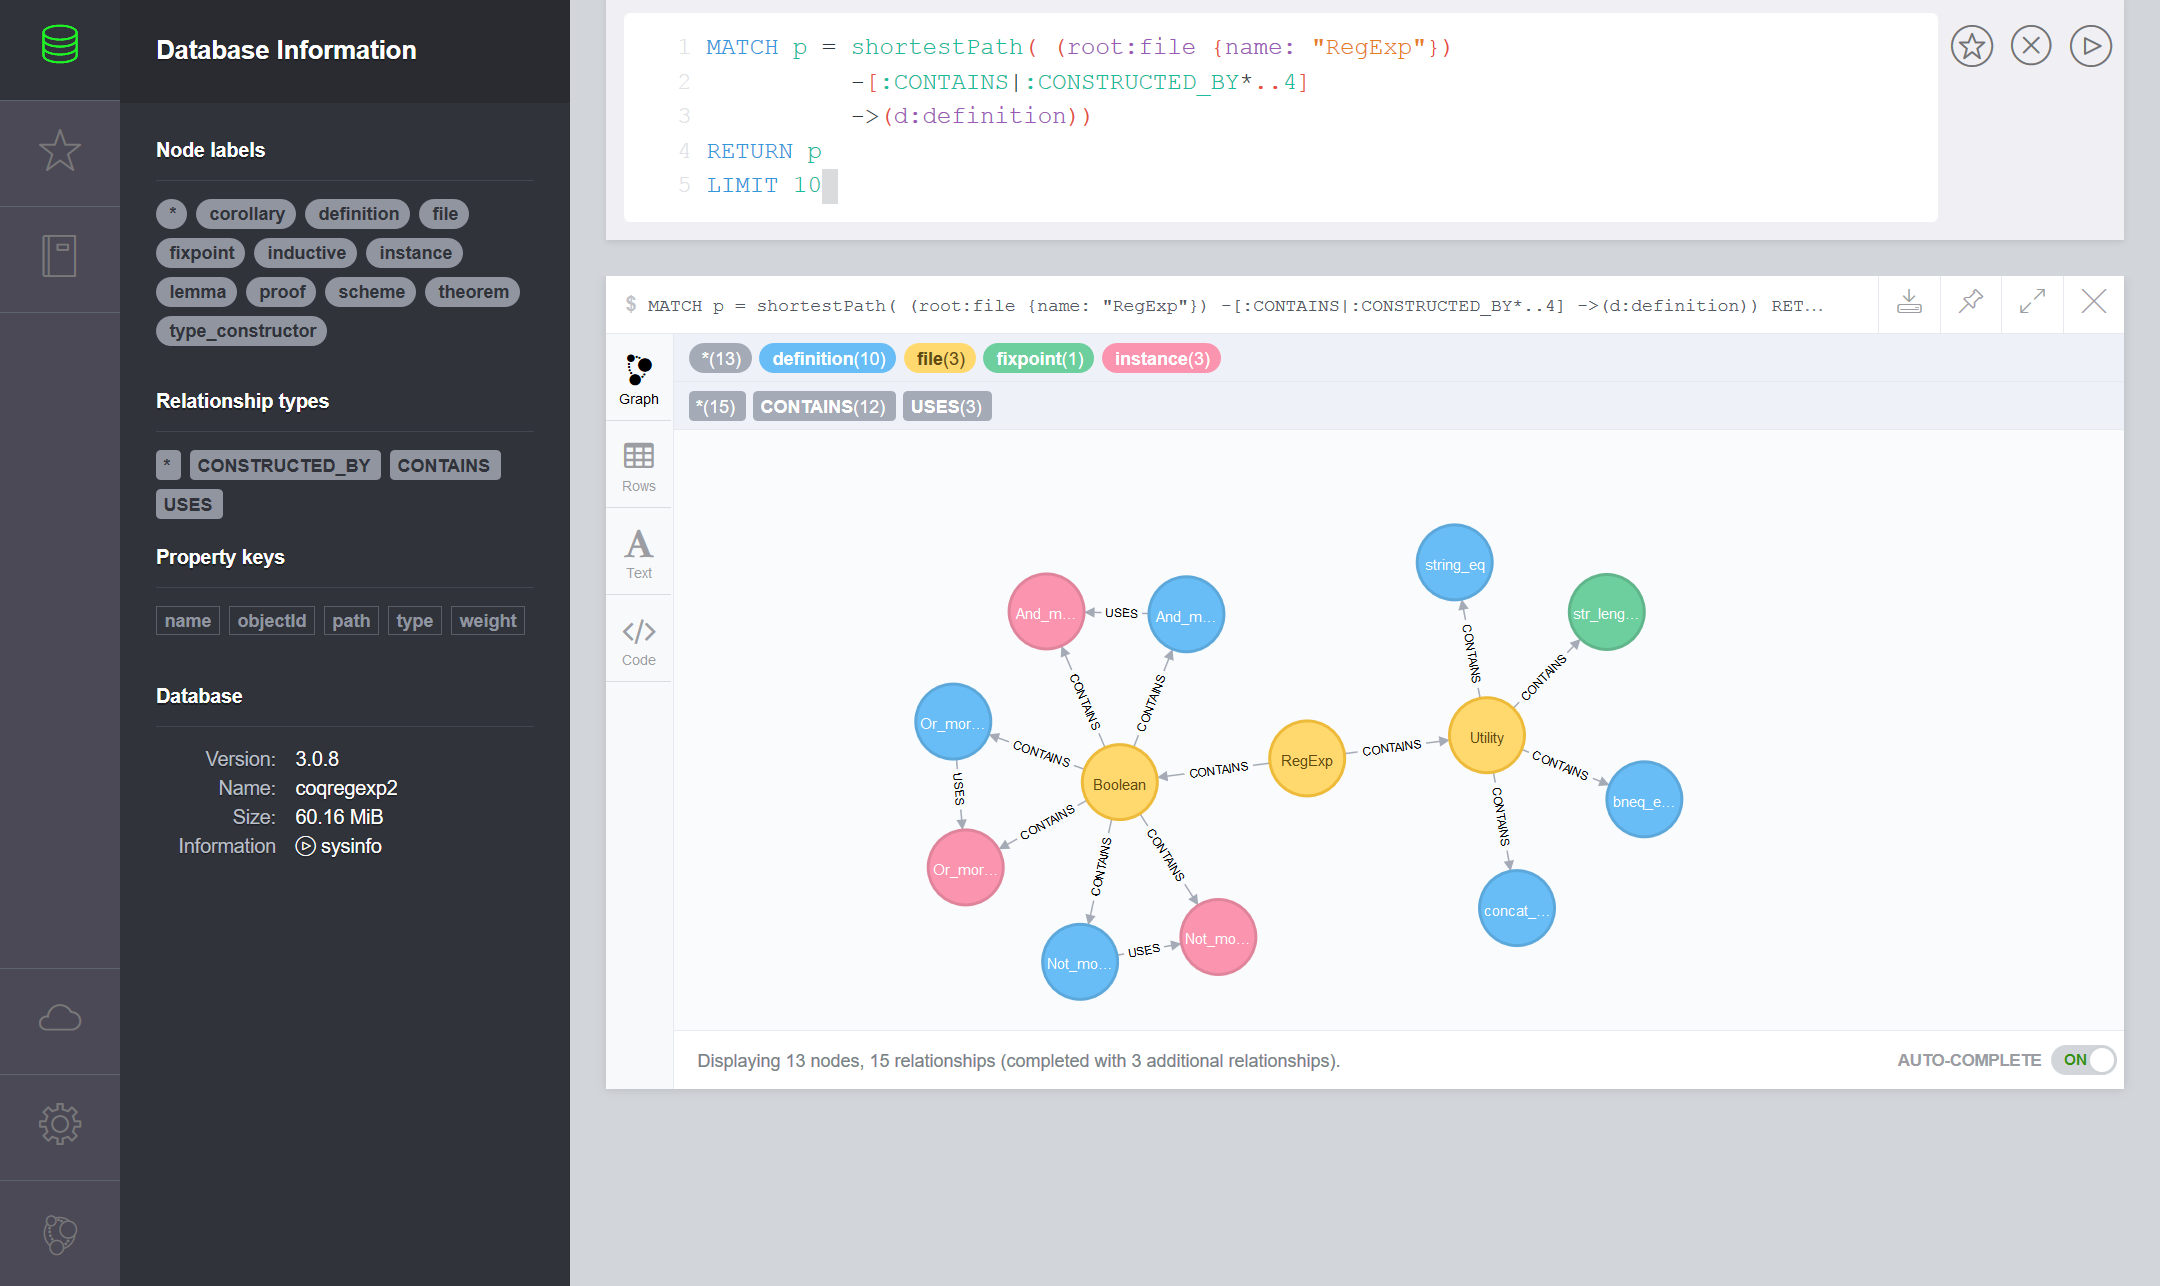
\includegraphics[width=\textwidth]{img/Neo4j_Browser.png}
  \caption{Neo4j Interactive Browser}
  \label{fig:neo4jbrowser}
\end{figure}

\subsection{Existing Tools for Neo4j}

\subsubsection{APOC: Awesome Procedures on Cypher}

\href{http://github.com/neo4j-contrib/neo4j-apoc-procedures}{\emph{Awesome
Procedures on Cypher}, or \emph{APOC}} for short, is a community-maintained Java
plugin featuring several graph algorithms callable from within Cypher itself.
Although there are other extension libraries (such as MazeRunner), APOC is well
documented, up-to-date and the most comprehensive, and therefore the obvious
choice as a foundation. By being a Java library hooked into Cypher, it offered
the potential for additional functionality to be built on top of it which
packaged-up some of the more complex features into \emph{domain-specific}
queries, intended for Coq users not familiar with Neo4j to get started with.
Thus, APOC helps step towards meeting the \emph{interaction} requirements for
this project by being easy to understand, flexibile to use and extensible; even
going part-way towards meeting the \emph{computation} requirements.

\subsubsection{igraph}

APOC has some key strengths that made it a good choice: it is easy to install
and use and has some basic graph algorithms to get started with.  However, its
main focus is on interacting with and combining different sorts and sources of
data and so lacks graph analysis functionality \emph{beyond} the basics. The
fact that it is implemented in Java further adds to its limitations: it is not
well-suited to more intense analyses over large graphs of libaries and is
insufficient to \emph{fully} meet the \emph{computation} requirements of this
project.

For such tasks, \href{http://www.igraph.org}{igraph} is ideal: it is described
on its website as a \emph{collection of network analysis tools, with the
emphasis on efficiency, portability and ease of use}. Written in C/C++ (with
bindings for R and Python), igraph offers a \emph{comprehensive} set of graph
algorithms without sacrificing on performance. These alogrithms and their uses
will be described later, in the Implementation chapter. For now, it suffices to
surmise that although igraph is not as easy to interact with (via the
statistics-oriented programming language R, as detailed in the next paragraph)
as APOC, the extra capabilities afforded were indispensible towards achieving
the \emph{computation} requirements of a core library of good defaults.

\subsubsection{visNetwork}

With igraph and APOC providing starting points for the computational aspects of
the projects, and the interactive Neo4j browser providing a well-polished,
graphical mode of interaction with basic, but useful, visualisation, the last
piece of the project was to incorporate the extra information gained from
\emph{executing} the graph algorithms.

\emph{Several} visualisation programs exist for Neo4j; however, many are for
commercial, industrial use and offer the features/complexity (and pricing) to
match. All tools which offer live visualisation with built-in Cypher query
execution (e.g. KeyLines, TomSawyer, Linkurious) are proprietary, requiring a
fee to use and offering more granularity than required. Offline (and
open-source) solutions (which require data to be exported in some manner before
visualisation) such as Gephi or Alchemy.js offer similarly many features, but at
the cost of a steep learning curve.  Ultimately,
\href{http://datastorm-open.github.io/visNetwork}{visNetwork}, (an R library
exporting to JavaScript which can be rendered inside a browser) was chosen due
to its simplicity and ease of integration with previous tools mentioned above.

\subsubsection{R}

\href{http://www.r-project.org}{R is a statistics-oriented programming language},
part of the Free Software Foundation's GNU poject. It is relevant for this
project because it offers an easy way to tie together Neo4j (through official
bindings), igraph and visualisation using visNetwork. This convenience came at
the price for having to learn R for this project, having been unfamiliar with it
prior. Nonetheless, it is a well-documented, relatively easy to pick-up language
and offered even more opportunities for learning during the course of this
project.

\section{Summary}

A detailed account into the planning of this project was given. The choice of
development methodology (spiral) and development tools (Git, GitHub, Travis-CI)
were noted. Requirements on modelling, interaction and computation were
explained and the choice of technologies and tools used as statrting points
(Coq, OCaml, dpdgraph, Neo4j, APOC, igraph, R and visNetwork) were justified
\emph{in relation} to \emph{which} requirements they satisfied.


\chapter{Implementation}

\guidance{%
  This chapter should describe what was actually produced: the programs which
  were written, the hardware which was built or the theory which was developed.
	Any design strategies that \textbf{looked ahead to the testing stage} might
	profitably be referred to (the professional approach again). 

  Descriptions of programs may include fragments of high-level code but large
  chunks of code are usually best left to appendices or omitted altogether.
  Analogous advice applies to circuit diagrams. 

  \textbf{Draw attention to the parts of the work which are not your own}. Making
  effective use of powerful tools and pre-existing code is often laudable, and
  will count to your credit if properly reported. 

  It should not be necessary to give a day-by-day account of the progress of the
  work but \textbf{major milestones may sometimes be highlighted with advantage}.
}

\prechapter{%
	Upon completion of the project's plan, its execution commenced. What
	follows is an account of the programs written, problems encountered, solutions
	implemented and tests conducted using the project-structure shown in
	Figure~\ref{fig:structure} as a guide. \emph{Reasons} for design decisions
	(arrived at using \emph{formative} evaluation techniques) are detailed in the
	next chapter.
}

\begin{figure}[tb]

\centering
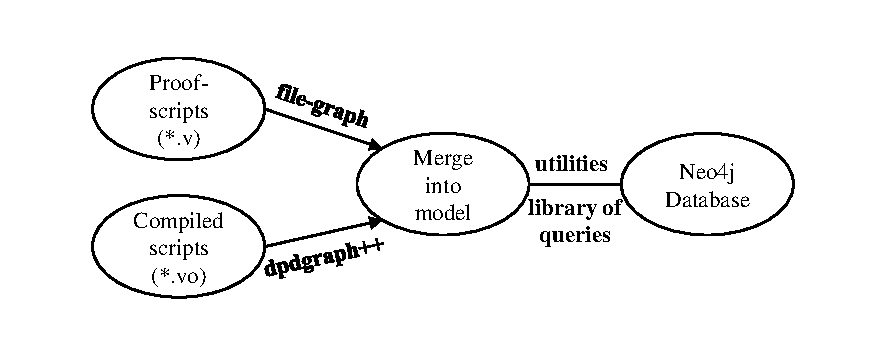
\includegraphics[width=\textwidth, page=1]{proposal/proposal-project-structure-diagram.pdf} 
\caption{System Components}\label{fig:structure}

\end{figure}


\section{Coq object-files to CSV}

This section of implementation corresponds to ``dpdgraph++'' on
Figure~\ref{fig:structure}: modelling the data contained in and the structure
of Coq object-files (\texttt{*.vo}) as comma-separated values (CSVs). The
initial model (inherited from the open-source ``dpdgraph'' tool) and subsequent
changes to it will be described.

\subsection{Modelling}

Initially, each edge was assigned a \emph{weight} representing the number of
(directed) uses of one node by another. Each node was assigned four
\emph{properties}: 

\begin{itemize}
  \item \emph{body}, a boolean representing whether a global declaration was
    either transparent or opaque;
  
  \item \emph{kind}, a ternary value representing whether a \emph{global
    reference} (a kernel side type for all references) was a reference to either
    the environment, an inductive type a constructor of an inductive type;

  \item \emph{prop}, a boolean value representing whether a term is a \texttt{Prop}
    (a decidable, logical property about a program, as opposed to a
    \texttt{Type});

  \item \emph{path}, a string value represent the module an object is in.
\end{itemize}

These ``properties'' were difficult to understand: they are not in the
vocabulary of a Coq programmer (e.g. \texttt{Definition}, \texttt{Inductive},
\texttt{Theorem}) and could not represent the richness of the
AST appropriately. It was not documented how to translate these constructs back
to familiar terms and thus, it quickly became clear that the these properties
needed to be replaced by more general and descriptive ones.

\subsubsection{Precise Kinds}

Apart from \emph{path}, all the properties were removed and replaced by two
\emph{labels}: labels are used to group  nodes into subsets; since a node can
belong to more than one subset, it can have more than one label assigned to it.
Implementation of this was straightforward: simply a matter of looking up and
expanding the abstract syntax tree starting from the type
\texttt{global\_reference}.

The two labels are \emph{kind} and \emph{subkind}.  A kind is a string which can
take one of the following values, each directly corresponding to an AST term:
\textsf{module}, \textsf{class}, \textsf{type\_constructor},
\textsf{inductive\_type}, \textsf{definition}, \textsf{assumption} or
\textsf{proof}.

Optionally, some terms have \emph{subkinds}, for distinguishing different
constructs more precisely. For example, when writing Coq, there is no
\texttt{Proof} keyword; instead \texttt{Theorem}, \texttt{Lemma}, \texttt{Fact},
\texttt{Remark}, \texttt{Property}, \texttt{Proposition} and \texttt{Corollary}
all are \emph{synonyms} for proofs. Full details can be found in
Appendix~\ref{chapter:fullmodel}.

\subsubsection{Recursive Modules}

What remained from the initial model was the \emph{path} property. The issue
here was that an inherently \emph{hierarchical} structure (of inclusion) was
represented \emph{flatly} as a string. This made modules second-class citizens,
not subject to the same analyses and manipulations as proof-objects, excluding
the possibility of expressing \emph{module-level dependencies} (as possible
in the coqdep tool).

Adding modules as 

Intention, execution, problems (remember the stack overflow), solutions.

\subsubsection{Types}

\subsubsection{Relationships}

\begin{itemize}
  \item Tried and \emph{removed} x\_USED\_BY\_y
  \item USES
  \item CONTAINS
  \item CONSTRUCTED\_BY
  \item Emphasis on direction of arrow for exploration, importance of consistency
\end{itemize}

\subsection{Translation}

\section{Coq source-files to CSV}
Intention, execution, problems, solutions.

Also, how it fit in with larger, open-source projects.

\subsection{Missing Information}

\subsection{Collection}
Explain Glob Files.

\subsection{Merging}

\section{CSV to Neo4j}
Intention, execution, problems, solutions.

Also, how it fit in with larger, open-source projects.

\subsection{Neo4j Import Tools}

\subsection{Impact of Changes to Model}
Trade-offs, execution.

\section{Query Library}
Intention, execution, problems, solutions.

Also, how it fit in with larger, open-source projects.

\subsection{APOC}

\subsection{Additions on top of APOC}

\subsection{igraph}

\subsubsection{Terminology}

\subsubsection{Betweenness Centrality}

\subsubsection{Closeness Centrality}

\subsubsection{PageRank}

\subsubsection{Community Detection}

\subsection{Visualisation}

\subsection{R Library}

\section{Project Related}
Modifying make files, testing, continuous-integration builds, editors

\section{Summary}
Features implemented, dead-ends and lessons learnt.


\chapter{Evaluation}\label{chapter:evaluation}

\guidance{%
  This is where Assessors will be looking for \textbf{signs of success} and for
  \textbf{evidence of thorough and systematic testing}. \textbf{Sample output},
  tables of timings and photographs of workstation screens, oscilloscope traces
  or circuit boards may be included.\\
  As with code, voluminous examples of sample output are usually best left to
  appendices or omitted altogether.\\
  There are some obvious questions which this chapter will address. \textbf{How
  many of the original goals were achieved? Were they proved to have been
  achieved? Did the program, hardware, or theory really work?}\\
  Assessors are well aware that large programs will very likely include some
  residual bugs. It should always be possible to demonstrate that a
  \textbf{program works in simple cases} and it is instructive to
  \textbf{demonstrate how close it is to working in a really ambitious case}.\\
}

\prechapter{%
  Here, the project's resounding success, in relation its aims (as listed in
  Section~\ref{intro:aims}), will be justified. A comparison with existing
  tools will demonstrate the advantages of this project over existing tools
  (those mentioned in Subsection~\ref{prep:coqtools}). Sample output will be
  shown and the interesting insights they provide will be explained.
}%

\begin{figure}[tbp]

  \raggedright
  This project aims to:

  \begin{itemize}
  \item represent Coq libraries as Neo4j graph databases, which wil involve
    \begin{itemize}
    \item exploring and choosing the correct model
    \item converting and extending existing code to output CSVs
    \item writing new programs to extract extra information \\
        (omitted from other, existing tools)
    \item writing new programs to automate database creation; and to
    \end{itemize}

  \item create a library of Neo4j queries, intended
    \begin{itemize}
    \item to highlight the structure of and relationship between proof-objects
    \item by coalescing and implementing several graph-related metrics.
    \end{itemize}
  \end{itemize}

  \hrule%
  \bigskip
  \caption{Aims of the Project}\label{fig:aims}

\end{figure}

\section{Features}\label{eval:compare}

For convenience, the aims of the project, as listed in
Section~\ref{intro:aims}, are reproduced above, in Figure~\ref{fig:aims}.
Within the first major bullet-point (representing Coq libraries as Neo4j
databases), the latter three aims (of adapting, extending and writing new
programs to output CSV, extracting extra information and automating database
creation) were exposited in the~\nameref{chap:impl} chapter.

So, to assess the first aim of the project (exploring and choosing the
correct model), all of the programs listed in
Subsection~\ref{prep:coqtools},~\nameref{prep:coqtools}, are compared
side-by-side in Table~\ref{table:features}, in which this project comes out
favourably.

\subsection{Other Tools}

\begin{table}[p]
  \centering

  \begin{tabular*}{\textwidth}{@{\extracolsep{\fill}} rcccccccccc}

    \toprule

    & \rot{Source Code} & \rot{Hyperlinks} & \rot{Precise Kinds}
    & \rot{Constr. \& Types~~} % for vertical space after 'Types'
    & \rot{Type Sig.} & \rot{Module depend.} & \rot{Graphical rep.}
    & \rot{Interactivity} & \rot{Statistics} & \rot{Object depend.} \\

    \midrule

    Coqdoc    & \Y & \Y & \Y & \Y & \Y & \N & \N & \N & \N & \N \\
    Coqdep    & \N & \M & \N & \N & \N & \Y & \Y & \N & \N & \N \\
    CoqSerAPI & \N & \N & \N & \N & \N & \N & \N & \Y & \Y & \N \\
    dpdgraph  & \N & \N & \M & \N & \N & \N & \Y & \N & \N & \Y \\
    Project   & \M & \Y & \Y & \Y & \Y & \Y & \Y & \Y & \Y & \Y \\

    \bottomrule

  \end{tabular*}

  \medskip
  \Y\  Has feature \hfill \N\ Does not have feature \hfill \M\ Can be extended to support it

  \bigskip
  \caption{Comparison of Features}\label{table:features}

\end{table}

\subsection{This Project}

It is clear from the table that this project either supports, or can support,
every feature supported by other tools. However, it is important to note, that
in many cases, this project does not simply match the feature, but exceeds it in
ways described next.

Linking to source code could be supported by modifying either the model,
database or JavaScript visualisations (outuput by the library of queries) to
link to the relevant webpages output by coqdoc. So, a user could switch between
a graphical overview and a detailed inspection at will.

Whenever a node is visible, it can be expanded to see the nodes it depends on,
so in that sense, it supports hyperlinks, though, unlike hyperlinks, such
expansion is done in place, thus retaining the \emph{context} of its use.

Thanks to the \emph{kind} and \emph{subkind} labels, the project supports
precise kinds.  Also, any (co-)inductive type can, via the
\texttt{CONSTRUCTED\_BY} relation, be expanded to see its constructors.

Due to the \emph{type} property, each object's type is also visible. For a proof
object, its type is a statement of the actual theorem being proved, hence this
feature is incredibly important when coming to grips with a mathematical theory.
Crucially, it is a \emph{fully expanded} type signature, making explicit any
assumptions introduced (perhaps hunderds of lines prior in the source code) into
the environment.

Module dependencies are set with the query in Listing~\ref{lst:moddep} by use of
the \texttt{CONTAINS} relation.  Interactivity is achieved through the Neo4j
browser interface and the JavaScript visualisations; statistics are achieved
through the library of queries; graphical representations by both. An important
limitation of CoqSerAPI is that its statistics are (at the time of writing)
simply three counters, whereas this project offers many sophisticated graph
metrics and the ability (through a queriable database) to gain \emph{any} sort
of information a user is interested in.

\begin{listing}[p]%

\caption{Query to set Module Dependencies}\label{lst:moddep}

  \begin{minted}{cypher}
    MATCH (a)-[:USES]->(b),
          (src:module)-[:CONTAINS]->(a),
          (dst:module)-[:CONTAINS]->(b)
    WHERE src.objectId <> dst.objectId
    CREATE UNIQUE (src)-[r:DEPENDS_ON]->(dst)
    SET r.weight = coalesce(r.weight, 0) + 1
    RETURN r
  \end{minted}

\end{listing}

And finally, object dependencies are at the heart of this project: by using a
Neo4j graph database, we can understand and manipulate this relation in a much
more flexible and scalable manner than any visualisation can manage.

\section{Performance}

This project could have all the features any user could ever want but if it ran
so slowly that nobody would have the patience to use it, then it would be wrong
to consider it as having met its aims. So, here, this project's execution time
is compared to most of the tools from the previous section. Although it is
slightly slower than other existing tools, this can be directly accounted for
by its larger feature set and increased flexibility.

\subsection{Setup}

To evaluate timings, the Coq (8.6) Standard Library was used, due to its sheer
size (564 modules, 5823 definitions, 23,892 proofs). For coqdoc and coqdep,
Coq's Makefiles were modified to measure execution time using bash's \emph{time}
command. At the time of writing, CoqSerAPI's statistics were not fully/usably
implemented, so it was not measured. For dpdgraph, seprate measurements were
taken for outputting a \texttt{dpd} file and converting that file to a dot
Format. A similar approach~\textendash of measuring database creation (model
output, CSV translation and data import) and library analysis
separately~\textendash was taken for this project, so that the comparison was as
fair as possible. Each set of timings was repeated five times (with the
exception of \texttt{dpd2dot} which, at nearly \emph{27 minutes}, was not
repeated because of time and system-usability constraints).

\begin{figure}[tp]
\centering
\begin{tikzpicture}[trim axis left]
	\begin{axis}[
    % width of chart
    width=\textwidth,
    % no box, below chart, horizontal
		legend style={%
      draw=none,
      at={(0.5,-0.15)},
      anchor=north,
      legend columns=3,
      column sep = 1em,
      cells={align=center},
    },
    % value above position on bar chart
		ybar=0.5ex, % bar chart, with inter-bar spacing of 1ex
    log ticks with fixed point,
    yticklabel={\pgfmathparse{pow(10,\tick-3)}\pgfmathprintnumber[fixed]{\pgfmathresult}}\,s, % N ms along y-axis
    symbolic x coords={User,System,Real},
		xtick=data,
    axis line style={opacity=0}, % hide y axis
    major tick style={draw=none}, % no ticks
    ymode=log, % log scale for y
    log basis y = {10}, % log base 10
		enlarge x limits=0.20, % spacing on x axis
    bar width=2ex,
    ymajorgrids, % rows of lines
    major grid style={white, line width=1pt},
    axis on top,
	]

  % Coqdoc
  \addplot [area legend, style={Blue,fill=Blue,mark=none}]
    coordinates {(User,7877) (System,0295) (Real,10007)};

  % Coqdep
  \addplot [area legend, style={red,fill=red,mark=none}]
    coordinates {(User,1361) (System,2299) (Real,4257)};

  % dpdgraph
  \addplot [area legend, style={LimeGreen,fill=LimeGreen,mark=none}]
    coordinates {(User,6872) (System,0645) (Real,9392)};

  % creation
  \addplot [area legend, style={Orchid,fill=Orchid,mark=none}]
    coordinates {(User,79254) (System,2521) (Real,98157)};

  % dpd2dot
  \addplot [area legend, style={ForestGreen,fill=ForestGreen,mark=none}]
    coordinates {(User,1272249) (System,2516) (Real,1588303)};

  % analysis
  \addplot [area legend, style={violet,fill=violet,mark=none}]
    coordinates {(User,255912) (System,49569) (Real,371881)};

  \legend{coqdoc,coqdep,dpdgraph,{model, CSV\\+ database},\texttt{dpd2dot},analysis}

	\end{axis}

\end{tikzpicture}

\caption{Comparison of Execution Times}\label{fig:exectimes}
\end{figure}

\subsection{Results}

Figure~\ref{fig:exectimes} shows the results of the comparison, as broken-down
by bash's time command into time spent in user-code, system calls and overall.
Note that the data is presented on a \emph{logarithmic} scale. Immediately
we see coqdoc takes very little time to run, approximately 10 seconds and coqdep
even less at around 4 seconds, which, considering their purely lexical
approaches, is to be expected.

So it is somewhat surprising that dpdgraph runs just as quickly as coqdoc. The
increase in system time can be explained by the 14MB \texttt{dpd} file output by
dpdgraph. Although at first it appears that there is an order-of-magnitude
slowdown with this project, more detailed examination explains precisely
\emph{what} occurs during database creation and where ineffeciencies lie.

\subsection{Inefficiencies}

Setting up a graph database from scratch can take some time. Assuming a Coq
project is already compiled, the following steps need to take place:

\begin{enumerate}
  \item\label{step:gen} generating file with a list of all the modules to be
    examined (15 ms),
  \item\label{step:compile} compile that file using the Coq compiler (12.6 s),
  \item\label{step:dpd2csv} convert the output \texttt{dpd} file to CSV files (72.7 s),
  \item create a Neo4j database from those CSV files (12.8 s)
\end{enumerate}

When steps~\ref{step:gen} and~\ref{step:compile} are taken on their own, we see
that the changes to accomodate a more detailed model resulted in a 25\%
slowdown, which is acceptable given this is a stress-test and the difference is
on the order of seconds. Creating a database from CSV files takes a similar
amount of time, also acceptable given the size of the graph (31,088 nodes and
850,434 edges).

So, the real bottleneck is step~\ref{step:dpd2csv}: converting \texttt{dpd}
files to CSV. During execution, \texttt{dpd2} reads in a 25MB \texttt{dpd} file
and outputs two CSV files of size 7MB (nodes) and 8MB (edges), so IO is likely
to be a factor, as is reconstructing the graph in memory. Outputting to
\texttt{dpd} was done to facilitate easy extension with other tools. It is
likely that outputting a CSV directly would have resulted in being able to
bypass this phase altogether, though, from a software-engineering
point-of-view, the trade-off there is increased coupling.

\subsection{Graph Analysis \& Visualisation}

Once a graph is created (whether it be in the form of \texttt{dpd} file or a
dabtabase) the last step is to \emph{use} the data by analysing and visualising
it. Here, this project shows a significant improvement over \texttt{dpd2dot}.

At nearly \emph{27 minutes}, its execution time dwarfs the analyses carried out
by this project. Whereas \texttt{dpd2dot} converted the output 13MB \texttt{dpd}
file to a 24MB dot file, in about one-quarter of the time, an R script was able
to run (a) PageRank and closeness centrality algorithms over all proofs and
defintions and (b) output \emph{8} different 9MB visualisations of the data.
Analyses took less than a minute; visualisations ranged from 20 to 90 seconds.

It should be noted that \texttt{dpd2dot} did not do graph \emph{layout}: it just
split the graph into subgraphs (based on modules) and assigned a colour and label
to each node (based on their properties). Converting the dot file to a viewable
format (e.g.\ a scalable vector-graphic or SVG) is up to another tool (that
being said, the command \texttt{dot -Tsvg} to produce an SVG visualisation had to
be cancelled after failing terminate within a few \emph{hours}).

\section{Library of Queries}\label{sec:libeval}

Within the second major bullet-point (creating a library of Neo4j queries), the
second aim (of coalescing and implementing graph-related metrics) was dealt
with in the~\nameref{chap:impl} chapter. To assess the first aim (of
highlighting the structure of and relationship between proof-objects), the
library will be shown to work on the small case of a Coq Regular-Expression
package and on the large case of the project's moonshot, the Odd Order Theorem.

\begin{figure}[p]
\centering
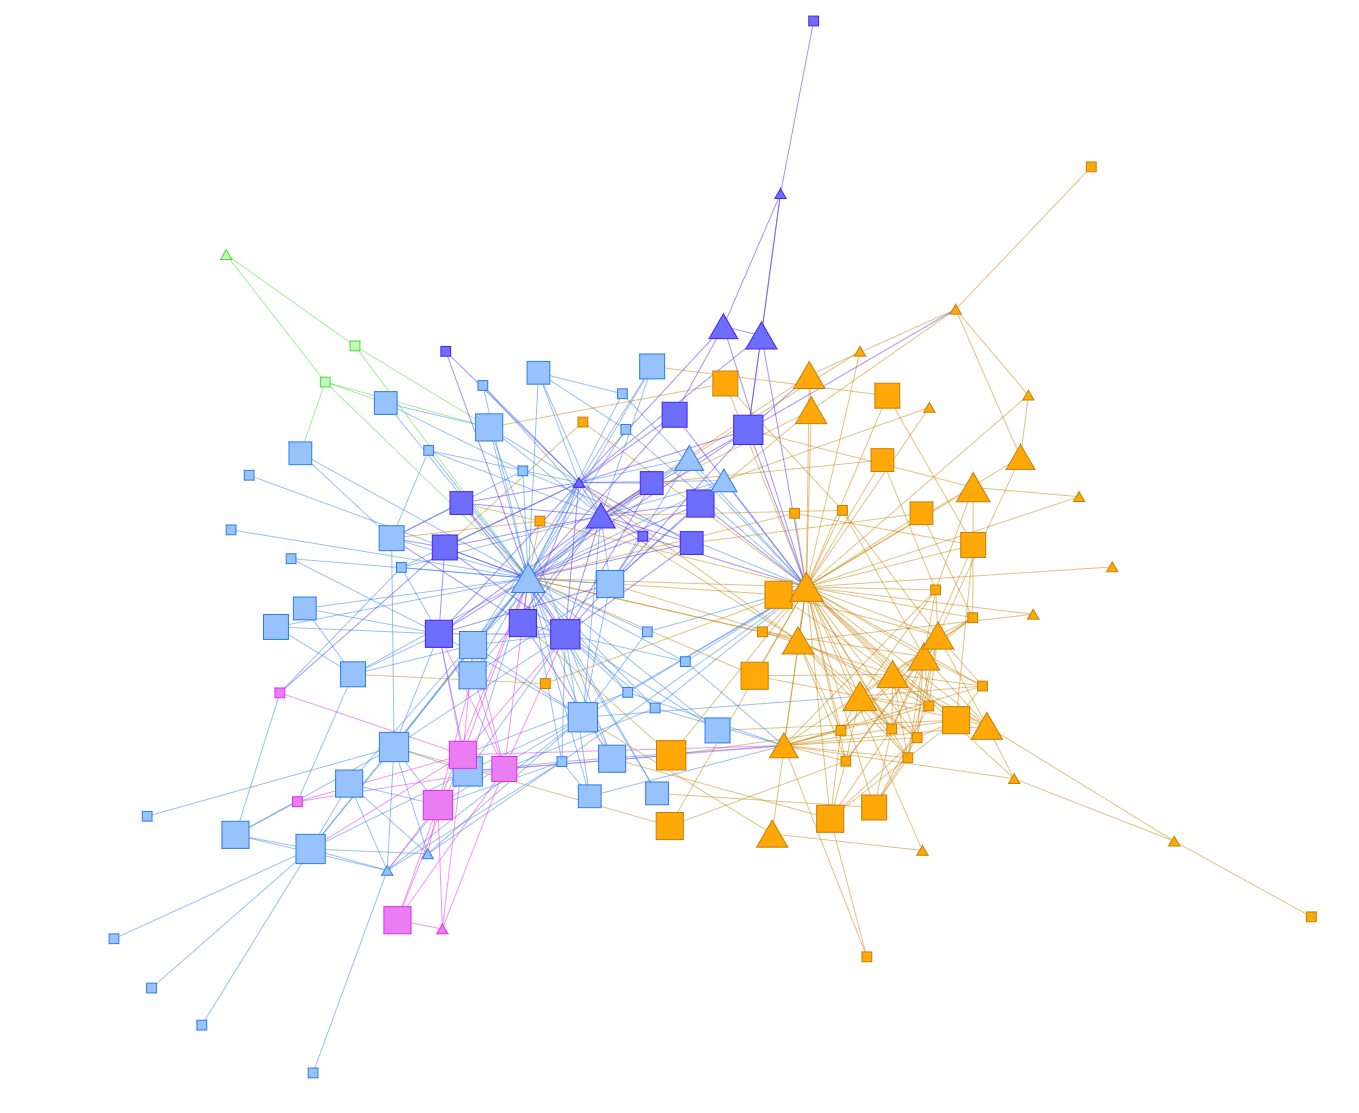
\includegraphics[width=0.8\textwidth]{img/regexp/direct.png}
\caption{Force-directed with Betweenness Centrality}\label{fig:regexp:direct}
\end{figure}

\begin{figure}[p]
\centering
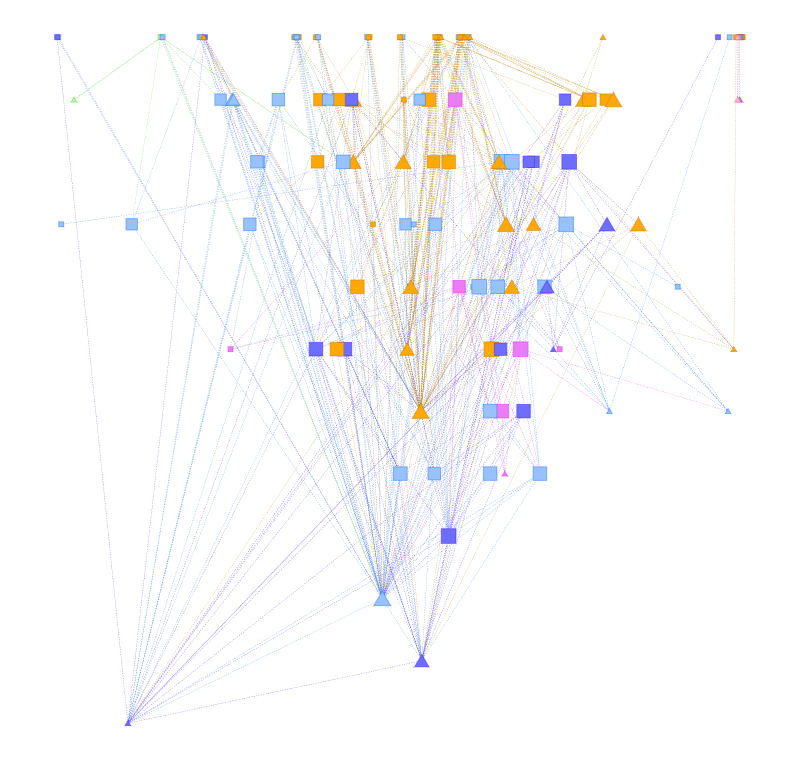
\includegraphics[width=0.8\textwidth]{img/regexp/hierarchical.png}
\caption{Hierarchical with Betweenness Centrality}\label{fig:regexp:hier}
\end{figure}

\begin{figure}[tp]
  \begin{minipage}{0.5\textwidth-0.5em}
    \centering
    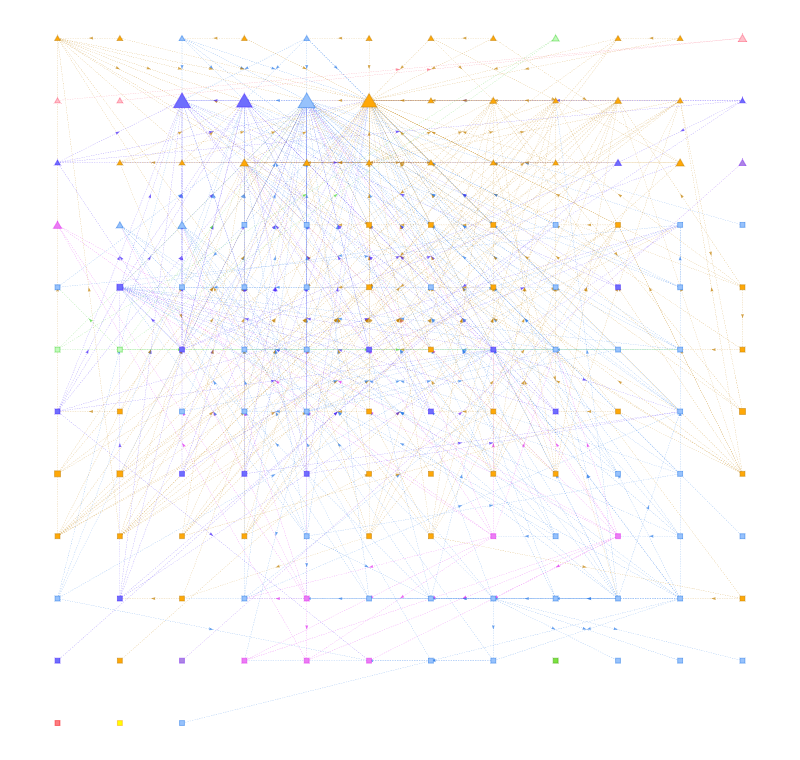
\includegraphics[width=\textwidth]{img/regexp/grid.png}
    \caption{Grid Layout with PageRank}\label{fig:regexp:grid}
  \end{minipage}%
  \hspace{1em}%
  \begin{minipage}{0.5\textwidth-0.5em}
    \centering
    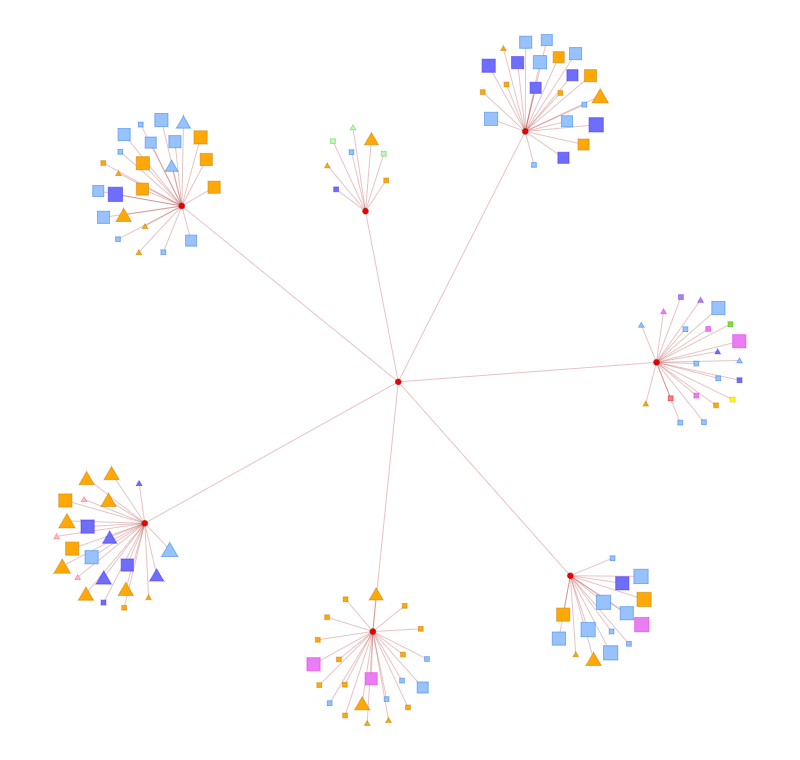
\includegraphics[width=\textwidth]{img/regexp/module.png}
    \caption{Force-directed with Modules}\label{fig:regexp:module}
  \end{minipage}
\end{figure}

\subsection{Small: CoqRegExp}

For this package, PageRank, betweenness centrality, modularity clustering,
hierarchical layout, grid layout and force-directed layout produced the most
aesthetically pleasing and insightful results. All graphs show only definitions
(shown as triangles, reminiscent of the $\triangleq$ symbol sometimes used for
definitions) and proofs (shown as squares, reminiscent of the end-of-proof
$\square$ symbol), except for Figure~\ref{fig:regexp:module} which also includes
modules (as circles).

\subsubsection{Direct}

Figure~\ref{fig:regexp:direct} shows a force-directed visualisation. The size of
the nodes corresponds to betweenness centrality scores (split up into 10
logarithmically equal-width buckets). Colours correspond to groups assigned by modularity
clustering. Edges represent the \texttt{USES} relation; edge-directions
(source-uses-destination) are omitted for clarity since they generally point
toward the the center of a cluster.

We see that modularity clustering largely corresponds to the how a human might
group nodes visually: two major clusters with a few, smaller clusters.
Intuitively, the \glblue{light blue} cluster represents \glblue{\emph{executable
functions}}; the \gorange{orange} cluster represents \gorange{\emph{proofs of
correctness}}; the \glpurple{light purple} cluster represents proofs using the
definition of \glpurple{string length}; the \glgreen{light green} cluster
represents proofs involving \glgreen{converting strings to regular-expressions};
the \gviolet{violet} cluster represents proofs relating to \gviolet{nullable
strings}. The node at the center of the light blue cluster is a function which
computes whether a given regular-expression matches a given string; the node at
the center of the yellow cluster defines what it means for two
regular-expressions to be equal.

\subsubsection{Hierarchical}

As far as insights are concerned, we see that this enables us to get a
high-level view of the threads of thought in the theory. We can see how these
threads develop by looking at Figure~\ref{fig:regexp:hier}.  Here, a Sugiyama
layout is used (the direction of edges always points downwards). If nodes were
partially ordered according the \texttt{USES} relation (destination $<$ source
if and only if source \texttt{USES} destination) then this layout ensures that
if a node (destination) is \emph{below} another node connected to it (source)
then the source \texttt{USES} destination.

Applied to mathematical theories, this layout is essentially a visual
study-guide, a plan for how to best tackle the material. It can be applied to
subgraphs, refined by declaring the maximum depth or the lowest layer to include
and filtered based on the kind or importance of a node.

\subsubsection{Grid and Modules}

Given a strategy for how to approach the material, knowing how important each
section is can be useful for gauging how much time to spend on understanding it.
As indicators of importance, measures of centrality are a useful way to do
precisely that. Figure~\ref{fig:regexp:grid} represents PageRank through node
size on uniform grid, useful for visually determining relative importance.

And finally, Figure~\ref{fig:regexp:module} shows the proofs and defintions
with modules, where edges represent the \texttt{CONTAINS} relation. We see that
the modules at the right and near the center (named Utility, Includes and Char
respectively) have very few important nodes (as determined by betweenness
centrality). Each module has two main parts: those relating to
\glblue{executable functions} those relating to \gorange{proofs of correctness},
occasionally accompanied by a few definitions/proofs on \gviolet{nullability}
or \glpurple{string length}.

\subsubsection{Insights}

Without studying even \emph{one line} of source code, we have been able to gleam
an intuitive and impressively detailed conceptual-scaffolding of this theory of
regular-expressions. A user can use the library of queries to futher explore the
theory or jump into reading the source code with a much better idea of how
the different pieces of the puzzle come together.

\subsection{Large: Odd Order Theorem}

For the Odd Order Theorem, betweenness centrality (for node size), modularity
clustering (for node colour), hierarchical layout, grid layout, circular layout
and force-directed layout produced the most aesthetically pleasing and
insightful results. As before, only definitions (shown as
triangles/$\triangleq$) and proofs (shown as squares/$\square$ symbol) are
shown, except for Figure~\ref{fig:oot:module} which also includes modules (as
circles). New to this section, edges are coloured. Unless a figure is stated as
being flipped, the colour of an edge is the same colour as its source (user);
otherwise, it is the same colour as its destination (used).

This Coq package closely follows the structure of the source material:
Peterfalvi~\cite{peterfalvi2000oot} and Bender \&
Glauberman~\cite{bender1994oot}. Each section (chapter) in the original books is
a file/module in the Coq package; each definition/lemma/proof/corollary
corresponds to the same in the books. Following the convention in the Coq
package, Bender \& Glauberman will henceforth be abbreviated to BG and
Peterfalvi to PF.

\subsubsection{Overview}

Starting with a force-directed visualisation of nodes,
Figure~\ref{fig:oot:direct} highlights five major groups: \gdblue{dark blue},
\gpink{pink}, \gyellow{yellow}, \gpurple{purple}, \gdgreen{dark green} and
\gmagenta{magenta}; it shows that modularity clustering largely agrees with the
layout. Clear connections are visible between each of the groups, with a central
group showing a mix of almost all groups.

Figure~\ref{fig:oot:module} shows the same nodes in their module structure; of
note is the remarkable consistency of clusterings (based \emph{only} on the
\texttt{USES} edges between proofs and definitions) to fall within their
grouping the moudule boundaries defined by the \texttt{CONTAINS} relation.

Figures~\ref{fig:oot:circleflip} and~\ref{fig:oot:grid} show a circular (with
edge directions flipped) and grid layout of the Coq package. An advantage of the
flipped circular layout is that is can show which groups are being used the most
and how; an advantage of the grid layout is one can get an intuition what
proportion of definitions/proofs belong to a certain group.

\subsubsection{Groups}

%  5 - Pink:        BG 1-6,AB
%  4 - Dark blue:   PF 1,2,5,6,7
%  3 - Purple:      BG 7,10,12,14,16 -- PF 3,4,8
%  1 - Dark green:  BG 7,8,9,10,11,12,13,15 -- PF 8,9,10,11,12,13,14,15
%  2 - Magenta:     BG 15,16 -- PF (1,8,9) 10,11,12,13,14
%  7 - Light green: BG (4,7) 10
% 20 - Yellow:      PF 3 - CyclicT Iso Reflection
%  6 - Light blue:  Stripped Odd Order

We can begin to uncover some of the meaning by looking at the \modulegraph.  The
seven \gpink{pink} circles (six near the center, one at the far left) are BG
sections 1-6 and Appendices A/B. As the first sections, one would assume they
lay the groundwork for the rest of the theory; this assessment is backed-up by
the \hiergraph. Of about 36 rows in the \gridgraph, 6 of them are \gpink{pink}.
All sections except BG 5 \emph{surround} the central cluster in the
\directgraph.  The slight red diagonal on the right of the \circlegraph\ shows
sparser connections than most of the other groups.

Similarly, the modules containing mostly \gdblue{dark blue} nodes are the early
chapters (1,2,5,6,7) of PF, expositing mostly foundational material (as seen in
the \hierflipgraph) but in an extremely directed and linear fashion (as seen in
the \hiergraph).  They are a dense group (as shown by the left of the
\circlegraph) and occupy about 6 rows in the \gridgraph. Apart from PF 2 (right)
and 5 (left), they are tightly-woven into the center of the \directgraph.

\gpurple{Purple} and \gdgreen{dark green} share the later sections (7-16) of BG.
Where they differ is PF: \gpurple{purple} covers PF 3,4 \& 8 whereas
\gdgreen{dark green} covers PF 8-15. This difference is apparent in
\hyperref[fig:oot:hier]{both} \hyperref[fig:oot:hierflip]{hierarchical} graphs:
\gpurple{purple} nodes occupy the middle of the graphs but green nodes form
a steep line from top to bottom. Both are clustered in the center of the
\directgraph, with the exception of PF 4 as two \gpurple{purple} clusters to the
bottom-left. They dominate the \circlegraph\ and the \gridgraph, occupying
around 8 rows each.

\gmagenta{Magenta} forms the later sections of both BG (15-16) and PF (8-14), so
it comes as little surprise that it occupies the upper half of both
\hyperref[fig:oot:hier]{both} \hyperref[fig:oot:hierflip]{hierarchical} graphs.
Even though it only constitutes about two rows in the \gridgraph, we see its
striking bands on the \circlegraph\ because of how often its results are used by
other nodes in the final sections (15-16) of PF.

Other miscellaneous groups include \glblue{light blue} (a self-contained,
stripped down proof of just the Odd Order Theorem from first principles),
\gyellow{yellow} (an entire excursion to proving PF Theorem 3.5) and
\glgreen{light green} (primarily BG 10).

\subsubsection{Insights}

With some context about the composition of the theory, we can now examine
\hyperref[fig:oot:hier]{both} \hyperref[fig:oot:hierflip]{hierarchical} graphs
in a bit more detail to see truly understand what they reveal about this
monumental Coq package and the books it encodes.

Figure~\ref{fig:oot:hier} shows the hierarchical, Sugiyama layout.  A
consequence of this algorithm is that nodes are placed \emph{closest to their
first use}, usually done as a heuristic to minimise edge crossings. Intuitively,
one can think of this approach as the lazy/ultra-efficient student who only
studies a particular definition/proof \emph{just before} it is needed by some
other part of the text (or like call-by-need evaluation in a non-strict
programming language).

As such, swapping the direction of the edges \emph{does not} simply flip the
layout vertically, as Figure~\ref{fig:oot:hierflip} shows. One could conjecture
that Figure~\ref{fig:oot:hier} shows how mathematics is \emph{developed} (a
narrow foundation, top-down refinement, creating proofs/definitions as and when
needed, several independent lines of thought) and Figure~\ref{fig:oot:hierflip}
shows how mathematics is presented (a broad base of \emph{all} the groundwork
that will be needed first, followed by a bottom-up, rapidly developing, linear
argument which uses the base extensively).

% Direct & Modules
\begin{figure}[p]
\centering
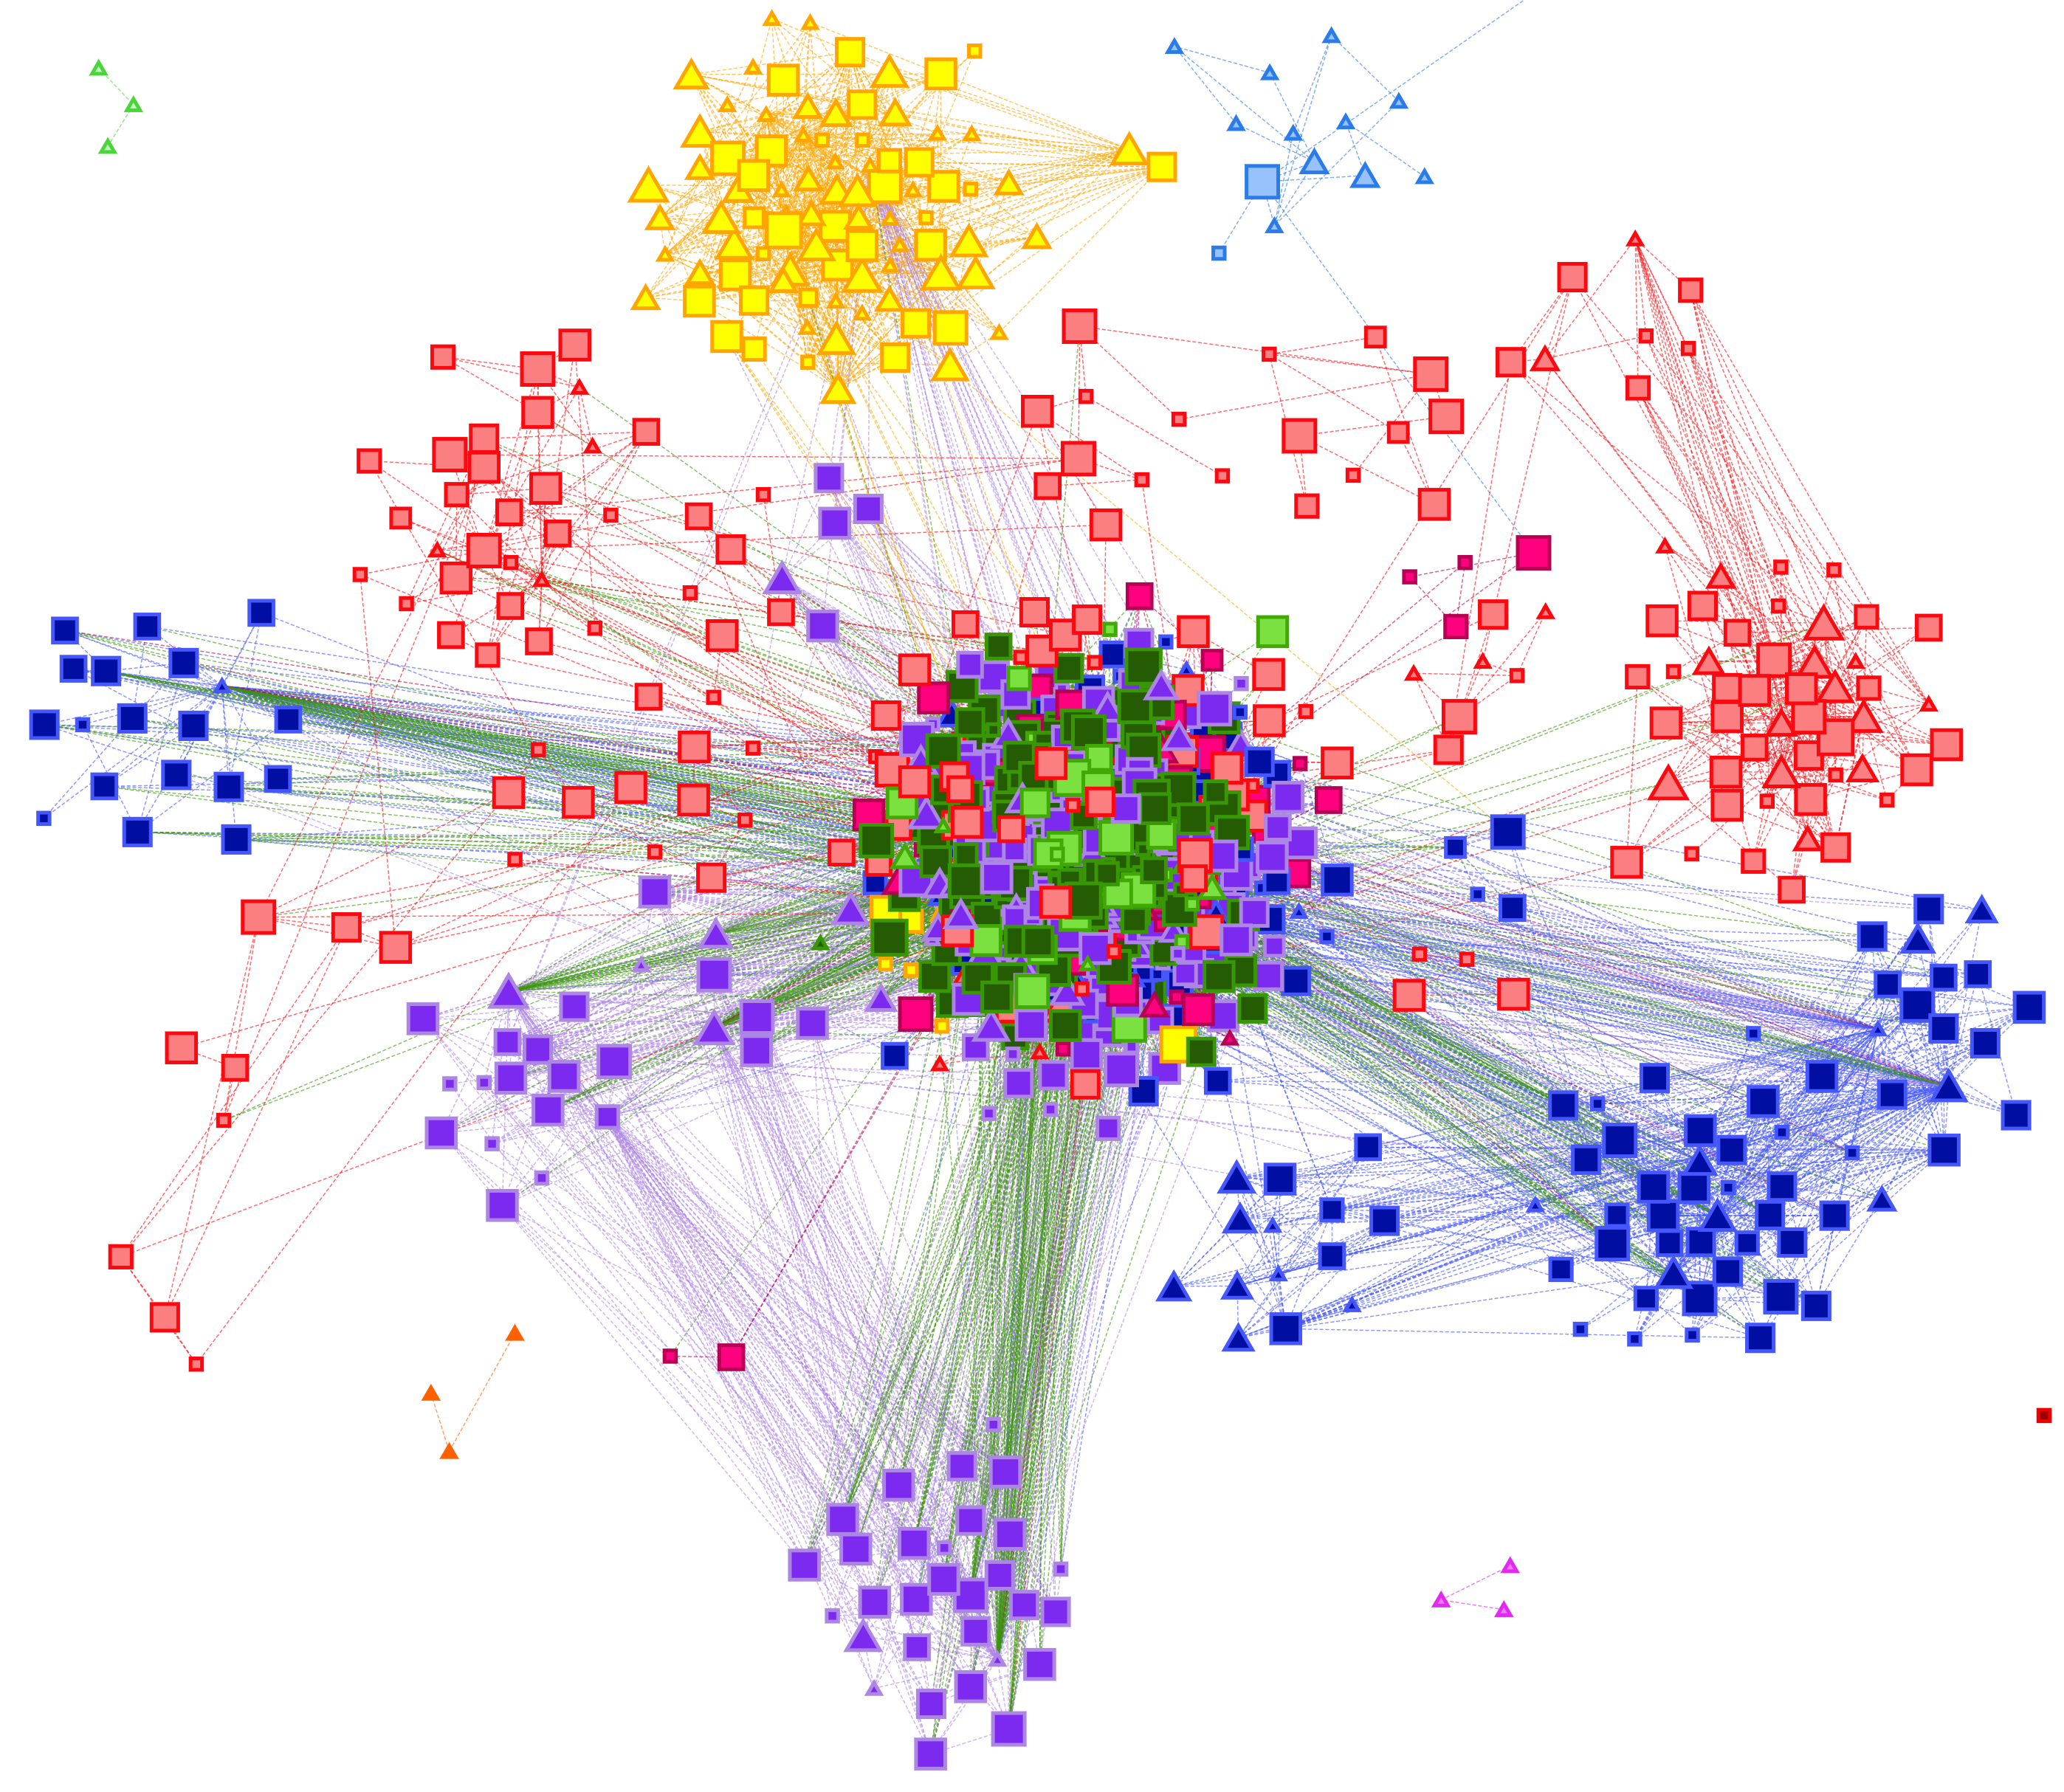
\includegraphics[height=0.45\textheight]{img/oot/direct}
\caption{Force-directed (some nodes omitted for clarity)}\label{fig:oot:direct}
\end{figure}

\begin{figure}[p]
\centering
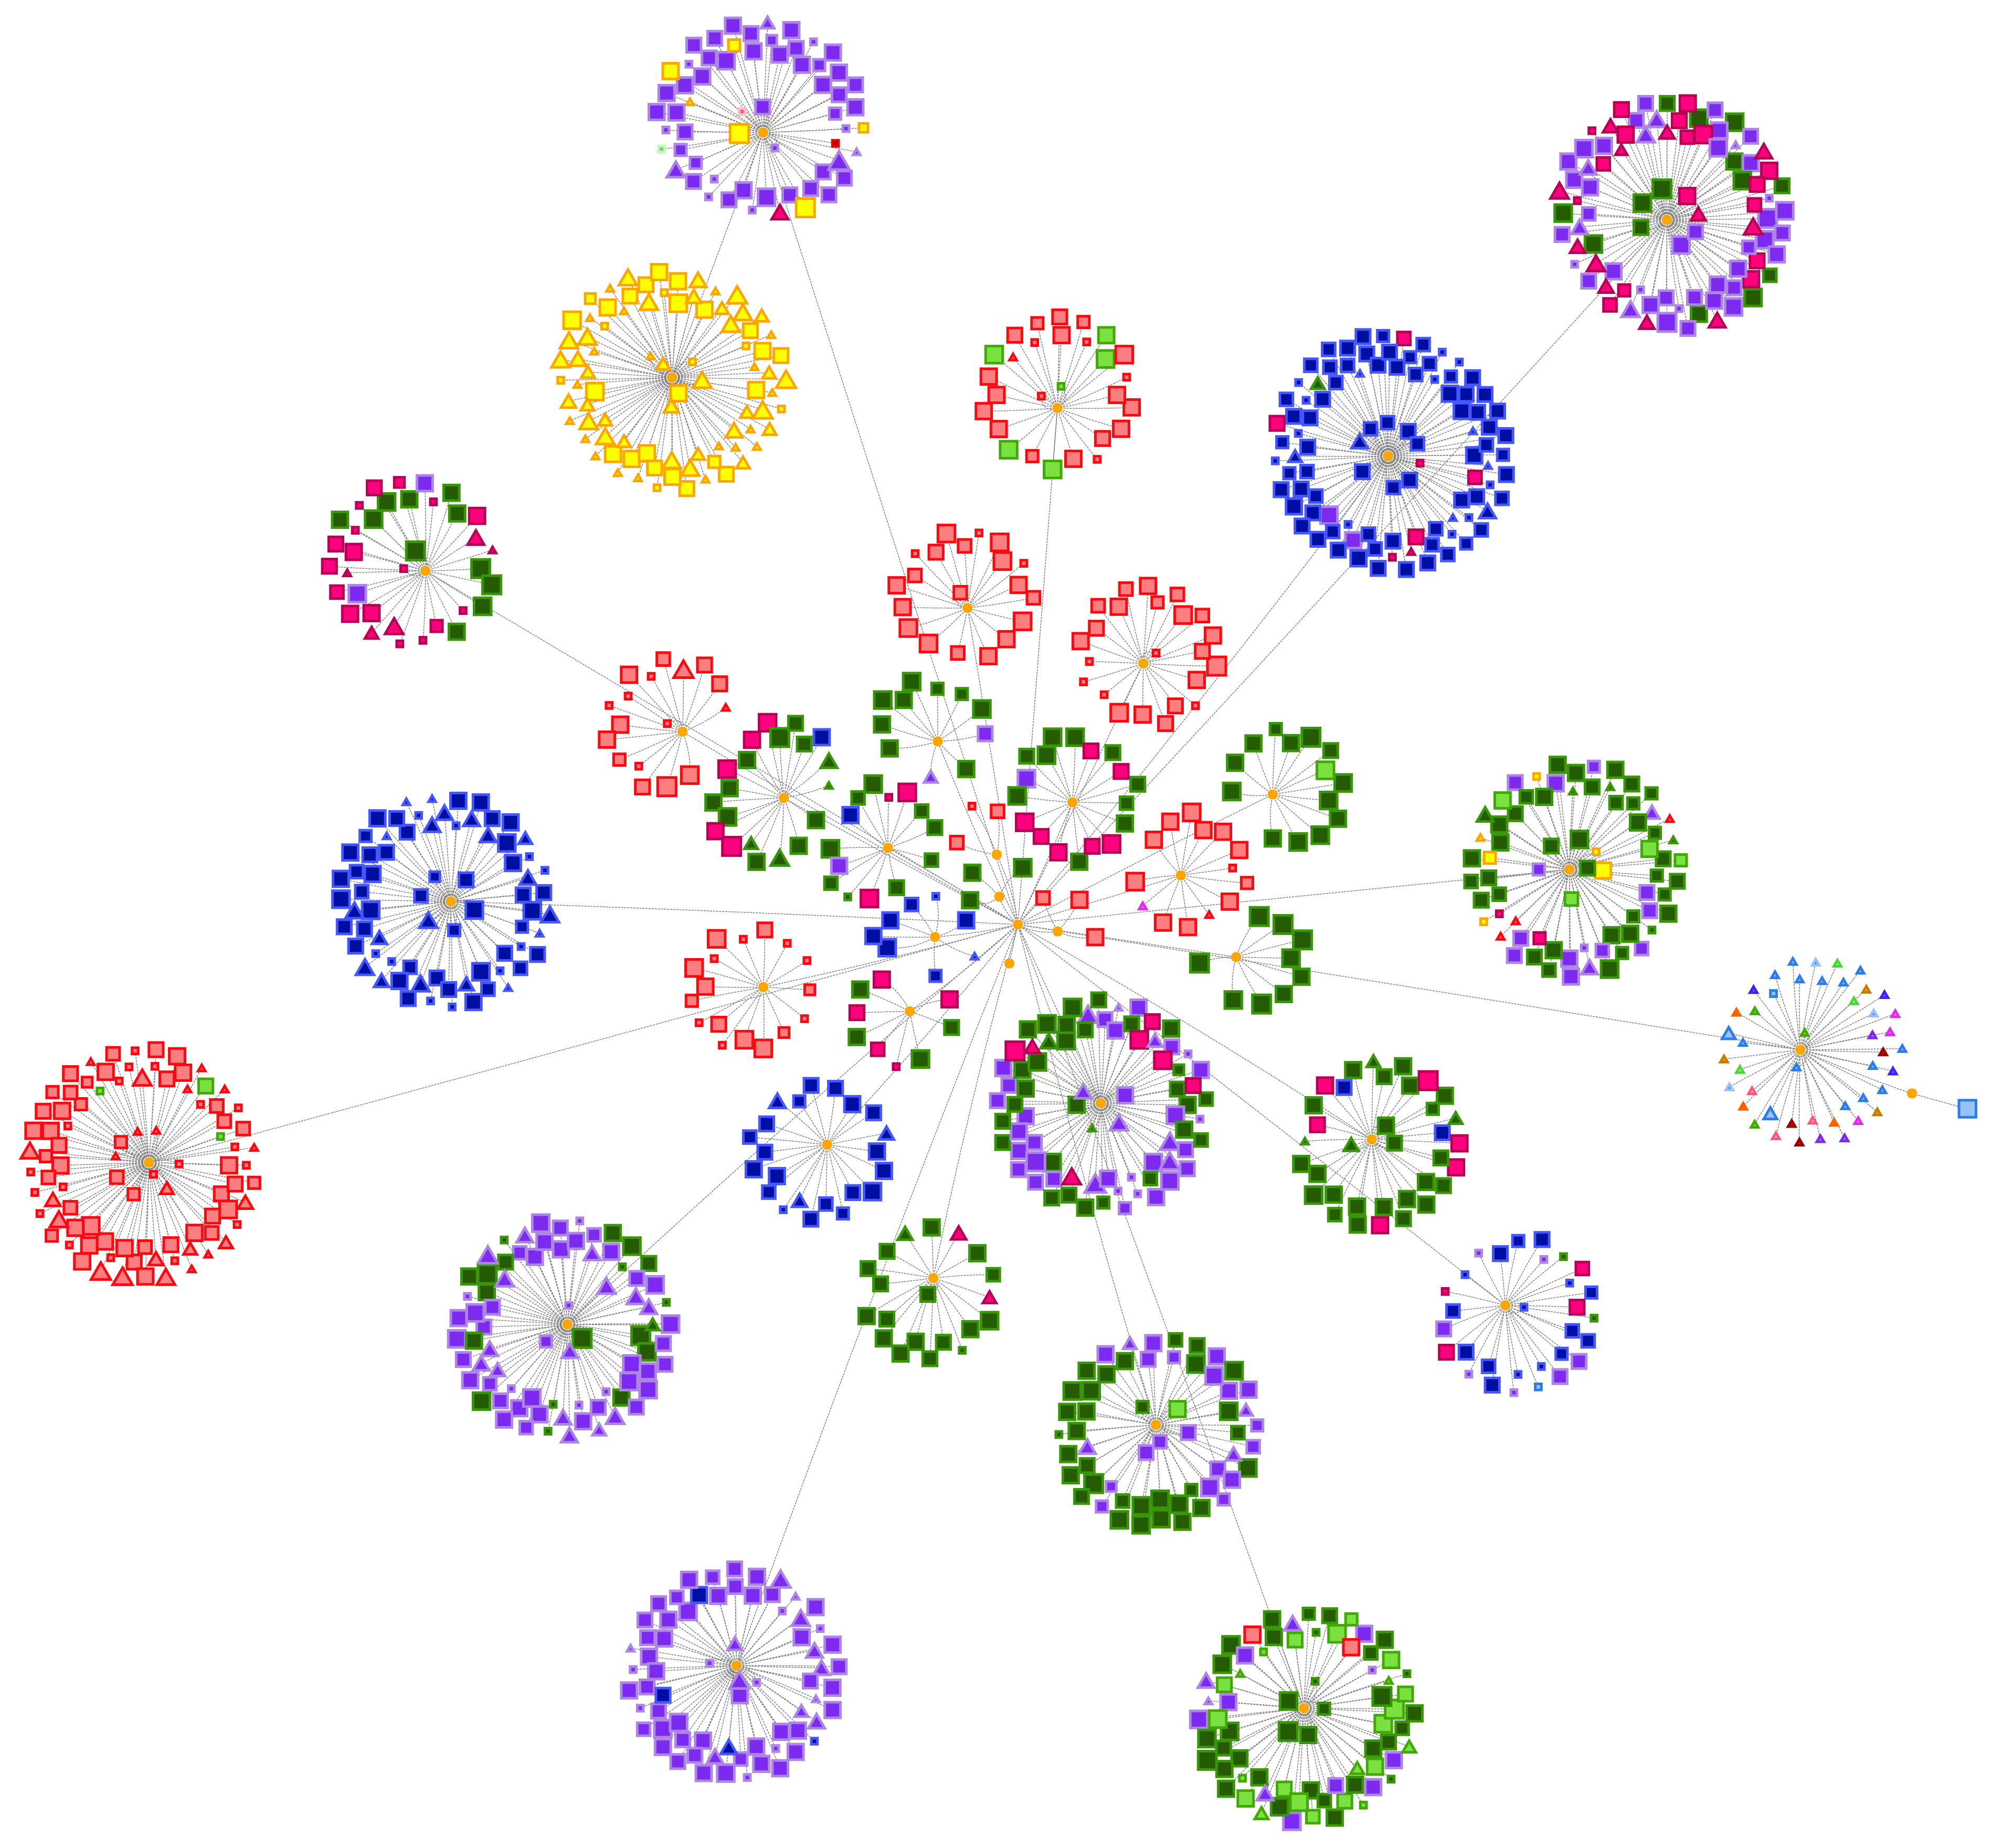
\includegraphics[height=0.45\textheight]{img/oot/modules}
\caption{Modules}\label{fig:oot:module}
\end{figure}

% Hierarchicals
\begin{figure}[p]
\centering
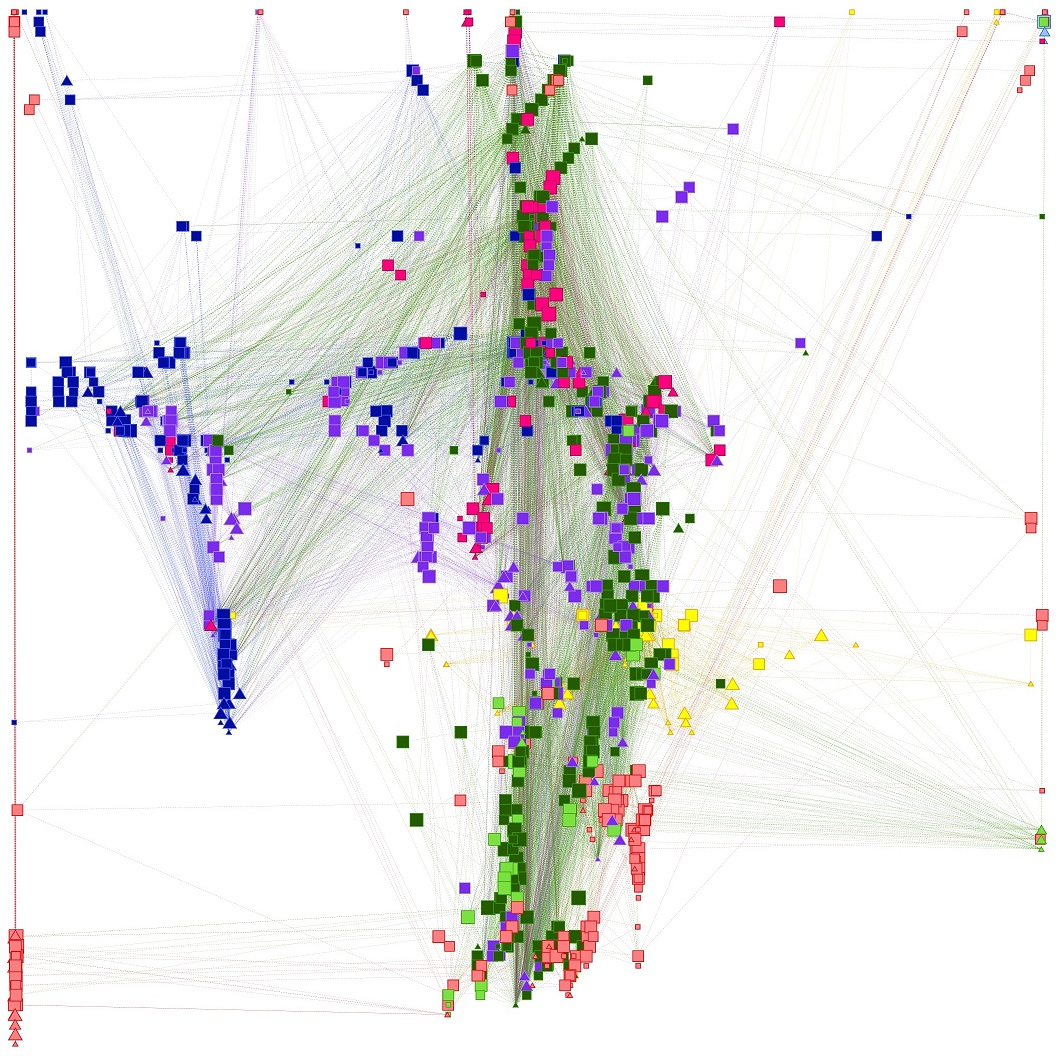
\includegraphics[height=0.45\textheight]{img/oot/hierarchical}
\caption{Hierarchical}\label{fig:oot:hier}
\end{figure}

\begin{figure}[p]
\centering
\reflectbox{\rotatebox[origin=c]{180}{%
  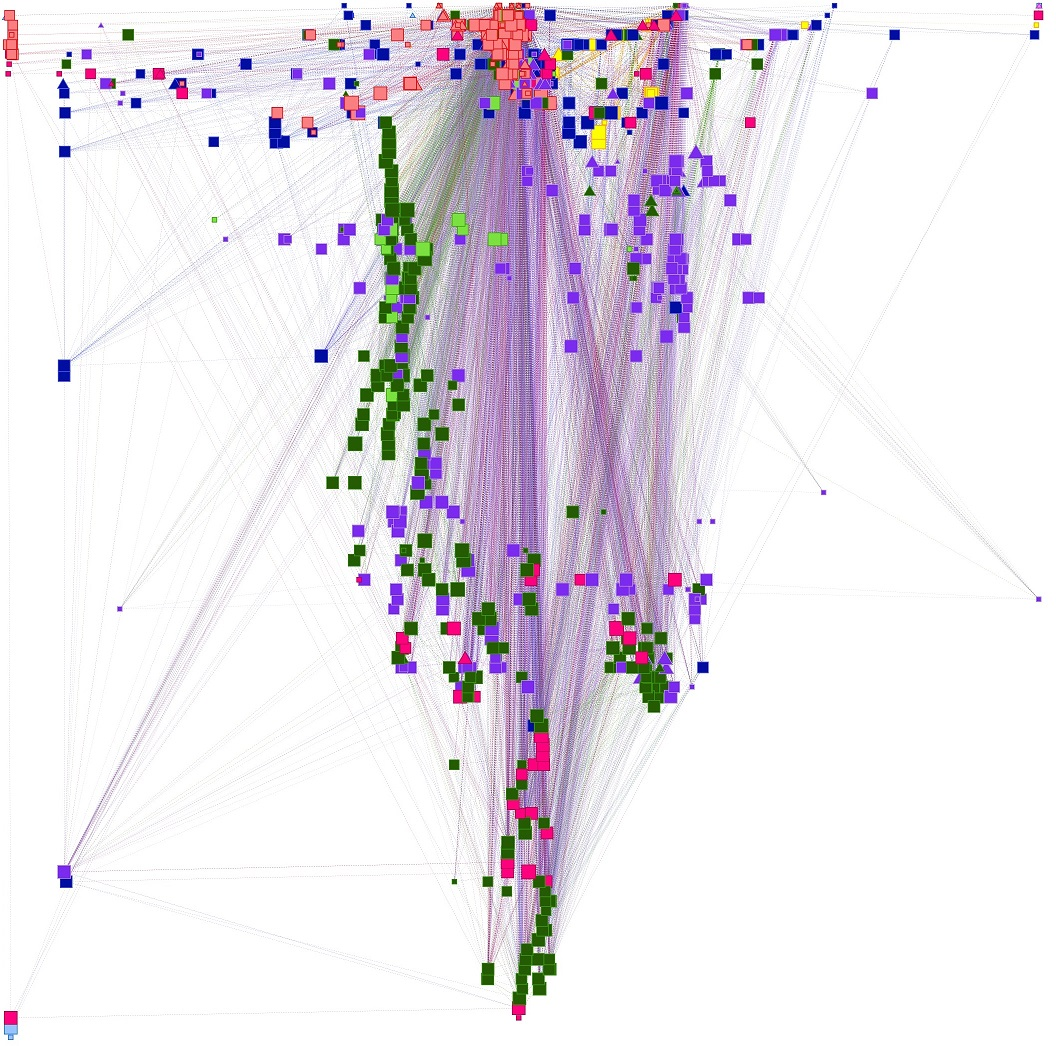
\includegraphics[height=0.45\textheight]{img/oot/hierarchical_flipped}}}
\caption{Hierarchical Flipped}\label{fig:oot:hierflip}
\end{figure}

% Circular & Grid
\begin{figure}[p]
\centering
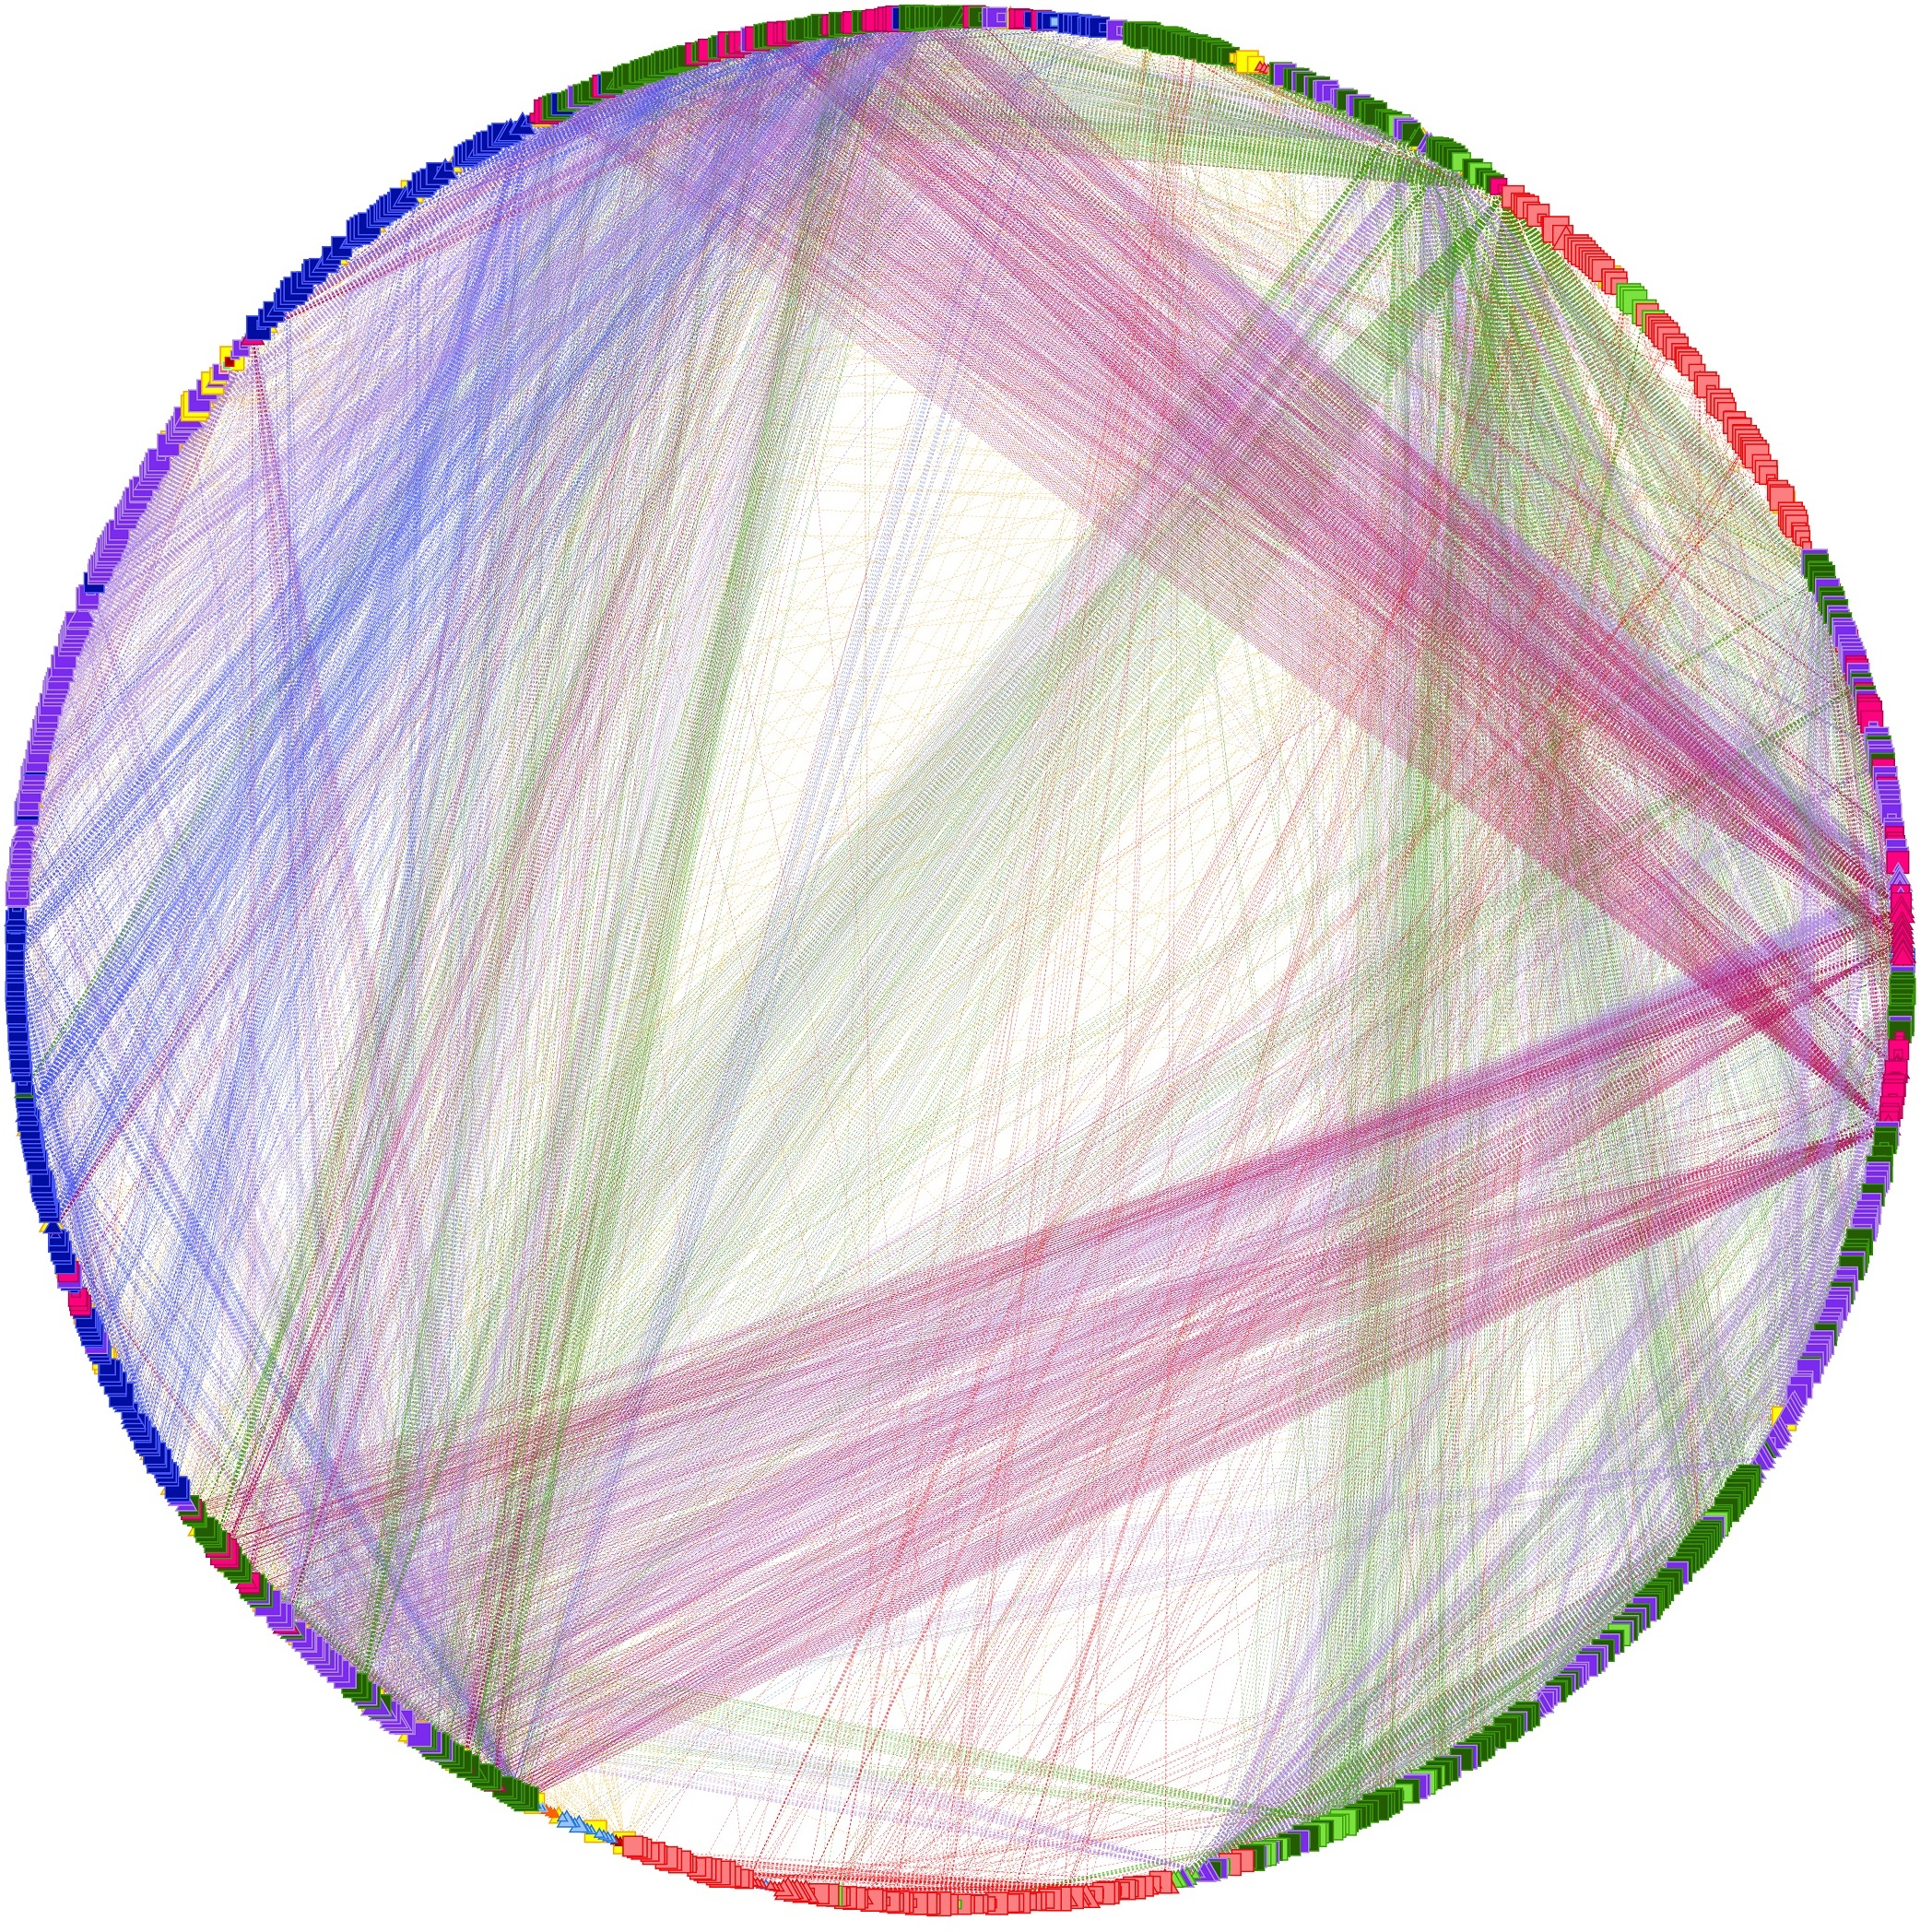
\includegraphics[height=0.45\textheight]{img/oot/circular_flipped}
\caption{Circular Flipped}\label{fig:oot:circleflip}
\end{figure}

\begin{figure}[p]
\centering
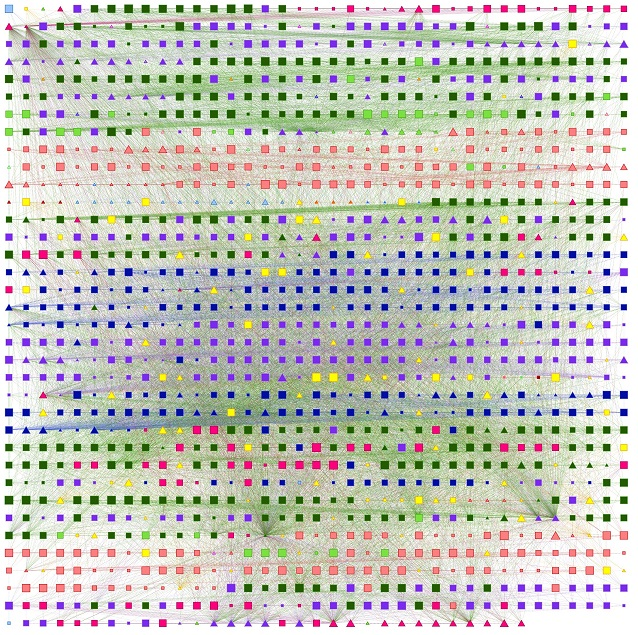
\includegraphics[height=0.45\textheight]{img/oot/grid}
\caption{Grid}\label{fig:oot:grid}
\end{figure}

\newpage%
\section{Summary}

To assess the two major aim of this project (choosing the correct model and
being able to gain insights into mathematical theories), its features,
performance and output were examined in detail. For its features, a systematic
comparison with other, existing tools of a similar purpose, showed this project
went above and beyond what existing tools offer. For its performance, a similar
comparison of execution times showed this project to be slightly slower, but
still acceptable and usable for even the most extreme of cases. For its output,
two Coq packages, each representing a mathematical theory, were explained via
the insights gained from using this project on them.


\chapter{Conclusions}

\section{Summary}

\section{In Hindsight}

\section{Future work}


\cleardoublepage{}
\phantomsection{} % Stop hyperlinks from going to the wrong page
\addcontentsline{toc}{chapter}{Bibliography}
\bibliographystyle{plain}
\bibliography{src/dissertation.bib}
\cleardoublepage{}

\appendix
\chapter{Full Model}\label{chapter:fullmodel}

Here is the full translation of the Coq AST to kinds and subkinds.

\begin{minted}[linenos,obeytabs=true,tabsize=2]{ocaml}
let kind_of_constref =
let open Decl_kinds in function
| IsDefinition def -> ("definition", Some (match def with
  | Definition -> "definition"
  | Coercion -> "coercion"
  | SubClass -> "subclass"
  | CanonicalStructure -> "canonical_structure"
  | Example -> "example"
  | Fixpoint -> "fixpoint"
  | CoFixpoint -> "cofixpoint"
  | Scheme -> "scheme"
  | StructureComponent -> "projection"
  | IdentityCoercion -> "coercion"
  | Instance -> "instance"
  | Method -> "method"))
| IsAssumption a ->
  ("assumption", Some (match a with
  | Definitional -> "definitional"
  | Logical -> "logical"
  | Conjectural -> "conjectural"))
| IsProof th ->
  ("proof", Some (match th with
  | Theorem -> "theorem"
  | Lemma -> "lemma"
  | Fact -> "fact"
  | Remark -> "remark"
  | Property -> "property"
  | Proposition -> "proposition"
  | Corollary -> "corollary"))

let kind_of_ind ind =
let (mib,oib) = Inductive.lookup_mind_specif (Global.env ()) ind in
if mib.Declarations.mind_record <> None then
  let open Decl_kinds in
  begin match mib.Declarations.mind_finite with
  | Finite -> "recursive_inductive"
  | BiFinite -> "recursive"
  | CoFinite -> "corecursive"
  end
else
  let open Decl_kinds in
  begin match mib.Declarations.mind_finite with
  | Finite -> "inductive"
  | BiFinite -> "variant"
  | CoFinite -> "coinductive"
  end

let get_constr_type typ =
  Names.KerName.to_string (Names.MutInd.user typ)

let kind_of_gref gref = 
if Typeclasses.is_class gref then
  ("class", None)
else
  match gref with
  | Globnames.ConstRef cst ->
  kind_of_constref (Decls.constant_kind cst)

  | Globnames.ConstructRef ((typ, _), _) -> 
  ("type_constructor", None)

  | Globnames.IndRef ind -> 
  ("inductive_type", Some (kind_of_ind ind))

  | Globnames.VarRef _ ->
  assert false


let kind_of_obj = function
| G.Node.Gref gref -> 
  kind_of_gref gref
| G.Node.Module modpath ->
      ("module", match modpath with
      | Names.ModPath.MPbound _ -> Some "bound"
      | Names.ModPath.MPdot _ -> Some "module"
      | Names.ModPath.MPfile _ -> Some "file")
\end{minted}

\cleardoublepage{}

\chapter{Project proposal}
% Conditional compilation
\providecommand{\setflag}{\newif \ifwhole \wholefalse}
\setflag

\documentclass[12pt,a4paper]{article}

\usepackage{booktabs} % Nice tables
\usepackage{graphicx}
\usepackage[top=1.1in, bottom=1.25in, left=1.25in, right=1.25in]{geometry}
\usepackage{hyperref}
\usepackage{xcolor}

% Remove ugly boxes around hyperlinks
\hypersetup{%
    colorlinks,
    linkcolor={red!80!black},
    citecolor={green!50!black},
    urlcolor={blue!80!black}
}

\parindent 0pt
\parskip 6pt

\begin{document}
\begin{center}
\Large
Computer Science Tripos -- Part II -- Project Proposal\\[4mm]
\LARGE
Exploring the structure of mathematical theories using graph databases\\[4mm]

\large
Dhruv C.~Makwana, Trinity College

Originator: Dr.~Timothy G.~Griffin

% \today
\end{center}

\vspace{5mm}

\textbf{Project Supervisor:} Dr.~Timothy G.~Griffin

\textbf{Directors of Studies:} Dr.~Frank Stajano \& Dr.~Sean B.~Holden

\textbf{Project Overseers:} Dr.~David J.~Greaves  \& Prof.~John Daugman

% Main document
\section*{Introduction and Description of the Work}
This project aims to (a) represent Coq libraries as Neo4j (graph) databases
and (b) create a library of Neo4j queries with the goal of highlighting
the structure and relationship between the representations of the proof-objects.

Mathematics textbooks aimed at professionals/researchers follow a well-established
rhythm: define some constructions and some properties on them and prove
theorems on both, with lemmas, corollaries and notation interspersed
throughout. Such a presentation is concise but limiting: it is linear; it forces
the reader to keep track of dependencies such as implicit assumptions, previously
defined results and the types and conventions behind any notation used;
and it offers little opportunity to consider and compare different approaches
for arriving at a result (i.e.\ number of assumptions, number of steps, some
notion of the importance of a result such as number of uses by later
results).

With the increasing popularity of interactive theorem-provers such as Coq
\cite{Coq:manual} and Isabelle \cite{nipkow2002isabelle}, many mathematical theories
(such as the formidably large Feit-Thompson Odd Order Theorem
\cite{peterfalvi2000oot, bender1994oot}) have been \cite{gonthier2013oot} or are being
translated and formalised into machine-checked proof-scripts. However, these
proof-scripts on their own inherit the same disadvantages as the aforementioned
textbooks, as well as some new ones: they are usually more verbose and explicit
and are primarily designed for automation/computation than readability. The
former (usually out of necessity to convey to the computer the intended
meaning) leads to unnecessary ``noise'' in the proof and the latter departs
from the vocabulary or flow a natural-language presentation may have.

The database world is currently experiencing a tremendous explosion of creativity
with the emergence of new data models and new ways of representing and querying
large data sets. \emph{Graph databases} have been developed to deal with highly
connected data sets and path-oriented queries. That is, graph databases are
optimised for computing transitive-closure and related queries, which pose a
huge challenge for traditional, relational databases.

A graph-based approach to the representation and exploration of the structure of
proof-objects would	be a far more natural expression of the complex
relationships (i.e.\ chains of dependencies) involved in
constructing mathematical theories. Questions such as ``What depends on this
lemma and how many such things are there?'' or ``What are the components of
this definition?'' could thus be expressed concisely (questions which are not
even expressible with standard relational databases systems such as
SQL). A popular graph database, Neo4j~\cite{neo4j} with an expressive query
language \emph{Cypher} will be used for this project.
	
\section*{Resources Required}

\subsection*{Software}
Several components of software will be required for executing this project, all
of which are available for free online.

For using the proof-scripts, the Coq proof assistant will be required, as well
as the Proof General proof assistant
(\href{http://proofgeneral.github.io/}{\texttt{proofgeneral.github.io/}}) for the Emacs
(\href{http://www.gnu.org/software/emacs/}{\texttt{www.gnu.org/software/emacs/}})
text-editor.

For writing the plug-in to access Coq proof-objects, the parser and associated
modules in the source code will be required
(\href{http://github.com/coq/coq}{\texttt{github.com/coq/coq}}) written in the OCaml
programming language (\href{http://ocaml.org}{\texttt{ocaml.org}}) with the OCaml's
Package Manager OPAM (\href{http://opam.ocaml.org}{\texttt{opam.ocaml.org}}).

For building the library of (Cypher) queries, Neo4j Community Edition will be
used.

\subsection*{Hardware}
Implementation and testing will be done on both Windows 10 and a Linux Virtual
Machine as appropriate and convenient on a Surface Pro 3 (Intel Haswell i7-4650U
1.7-3GHz, 8GB RAM, 512GB SSD) with a personal GitHub account and physical backup
drive (Seagate 1TB) making hourly backups using Windows' File History.

\section*{Starting Point}
Some existing tools offer part of the solutions: these will be used and
combined as appropriate. A large part of the project will rely on my knowledge of
OCaml and Coq usage and internals.

Coq-dpdgraph
(\href{http://github.com/Karmaki/coq-dpdgraph}{\texttt{github.com/Karmaki/coq-dpdgraph}})
is a tool which analyses dependencies between \emph{compiled} Coq proofs. As
such, desirable information about notation, tactics, definitions and the
relationship between a type and its constructors is lost.

Coqdep is a utility included with Coq which analyses dependencies \emph{at the
module level} by tracking {\tt Require} and {\tt Import} statements.

Coq SerAPI
(\href{http://github.com/ejgallego/coq-serapis}{\texttt{github.com/ejgallego/coq-serapis}})
is a work-in-progress library and communication protocol for Coq designed to
make low-level interaction with Coq easier, especially for IDEs. It has a
starting point for gathering some statistics of proof-objects in a project.

All of these tools have the same disadvantage: they present information statically,
with no way to query and interact with the information available.

\section*{Substance and Structure of the Project}
\begin{figure}[tb]
	\centering
	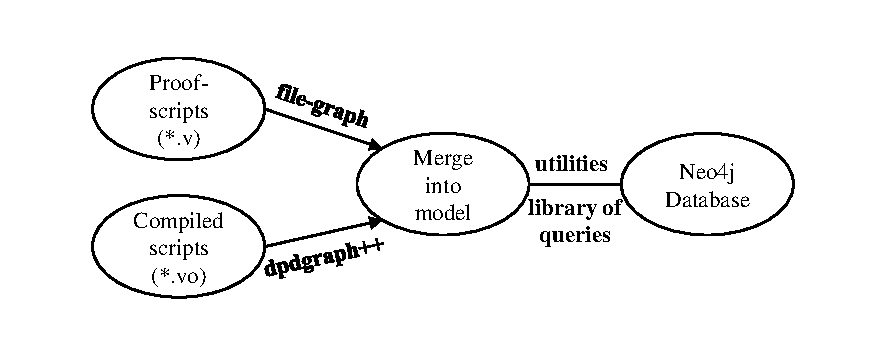
\includegraphics[width=\textwidth, page=1]{proposal/proposal-project-structure-diagram.pdf} 
  \ifwhole%
    \caption{System Components (repeated from page~\pageref{fig:structure})}
  \else
    \caption{System Components}\label{fig:structure}
  \fi
\end{figure}

The project will have three major parts, as shown in Figure~\ref{fig:structure}.

\subsection*{Processing Compiled Files}
First, using coq-dpdgraph as a starting point, a tool which expresses a
compiled proof-script as CSV files (shown as ``dpdgraph++'' in the diagram).
Finding what information can and should be extracted will be an iterative
process. Although coq-dpdgraph is functional, it is very basic with no way of
even relating the relationship between a (co-)inductive type and its
constructors, hence much work is to be done to even come close to utilising the
full potential of compiled proof-scripts.

\subsection*{Processing Source Code Directly}
Second, using Coq's sophisticated extensible-parser, to parse, gather and
convert to CSV files the desirable but missing information
coq-dpdgraph does not extract (shown as ``file-graph'' in the diagram). An
interesting feature of Coq's parser is that it allows new constructs and
notation to be defined: this is used heavily in some projects and therefore
poses a great challenge for simply understanding and using the parser
effectively.

\subsection*{Extraction and Analysis Tools}
Lastly, writing utilities to automate analysis of Coq files and importing them into
Neo4j and libraries of queries to run on imported data in Neo4j. Since it is not
known what sort of data can be extracted and what will be useful or interesting to
know, modelling the data -- in this case the structure and objects of a mathematical
proof -- will be an non-trivial task which will be tackled iteratively.

\subsection*{Extensions}

Extensions for this project will come from the process of adapting the project to
be compatible with SSReflect~\cite{gonthier2015ssr}, part of the Mathematical
Components set of tools for Coq. These set of tools use low-level hooks in the
Coq plugin system to significantly alter the specification and computation of
proofs. As such, although they allow for large-scale projects to be formalised
more easily, they are non-standard and would thus be very difficult to support
fully.

\section*{Success Criteria}
Alongside a planned and written dissertation describing the work done, the
following criteria will be used to evaluate the success of this project:

\begin{enumerate}

	\item A schema of attributes and relations for each proof-object is defined.
	\item Programs which convert proof-scripts and compiled proofs to CSV files
		  are implemented.
	\item A library of queries in order to manipulate and explore the proof-objects
		  is implemented.
	\item These new sets of tools are shown to have more capabilities and perform
		  comparably to existing tools for exploring mathematical theories.

\end{enumerate}

\newpage
\section*{Timetable and milestones}
\vspace*{\fill}

\begin{table}[h]
\centering
\begin{tabular}{ll}
    \toprule

    Date & Milestone \\

    \midrule

	% October
	21-10-2016	&	Complete Project Proposal \\ \\
          
	% November
	04-11-2016	&	Finish a prototype compiled-to-CSV tool. \\ 
				&	Get familiar with Neo4j Cypher. \\
				&	Understand how to use the Coq parser. \\ \\

	18-11-2016	&	Refine compiled-to-CSV tool: tests and documentation. \\
				&	Explore queries possible and start the library. \\
				&	Begin work on translating Coq constructs from proof-scripts. \\ \\

	% December
    02-12-2016	&	Finish a prototype script-to-CSV tool. \\ \\

    16-12-2016	&	Test and document script-to-CSV tool. \\ \\

    30-12-2016	&	Begin work on integrating tools into one workflow. \\ \\

	% January
	13-01-2017	&	Stabilise and document whole project so far. \\
				&	Prepare presentation for CoqPL Conference. \\ \\

    27-01-2017	&	Look at SSReflect and evaluate changes to be made. \\ \\

	% February
    10-02-2017	&	Incorporate changes from feedback/new features. \\ \\

    24-02-2017	&	Test and document the new features. \\ \\

	% March
	10-03-2017	&	Write Introduction, Preparation and Implementation chapters. \\ \\

    24-03-2017	&	Fix bugs/unexpected problems. \\ \\
    
	% April
    07-04-2017	&	Write Evaluation and Conclusion chapters. \\ \\

    21-04-2017	&	Fix bugs/unexpected problems. \\ \\
    
	% May
	05-05-2017	&	Complete Dissertation (references, bibliography, appendix, formatting). \\

  \bottomrule

\end{tabular}
\end{table}
\vspace*{\fill}

\ifwhole \else

  \newpage
  \phantomsection{} % Stop hyperlinks from going to the wrong page
  \bibliographystyle{plain}
  \bibliography{src/dissertation.bib}
  \cleardoublepage{}

\fi

\end{document}


\end{document}
